\documentclass[preprint,12pt]{elsarticle}

\usepackage{graphicx}
\usepackage{booktabs}
\usepackage{multirow}
\usepackage{amsmath}
\usepackage{siunitx}
\usepackage{subcaption}
\usepackage{float}
\usepackage[hidelinks]{hyperref}
\setlength{\tabcolsep}{4pt}
\graphicspath{{results/figures/}}

\makeatletter
\pdfstringdefDisableCommands{%
  \def\corref#1{}%
  \def\cortext#1{}%
  \def\@corref#1{}%
  \def\cnotenum#1{}%
}
\makeatother

\sisetup{
  round-mode = places,
  round-precision = 3
}

\journal{Computer Methods and Programs in Biomedicine}

\begin{document}

\begin{frontmatter}

\title{A Reproducible Within-Corpus Audit Framework for Melanoma Classification Integrating Segmentation, Calibration, Decision-Curve Analysis, and Explainability}

\author[inst1]{Rafael Oliveira Chaves\corref{cor1}}
\author[inst2]{Antonio Pereira Junior}
\cortext[cor1]{Corresponding author: rafael.ufpa@gmail.com}

\address[inst1]{Institute of Technology, Federal University of Pará, 66075-110 Belém (PA), Brazil}
\address[inst2]{Signal Processing Laboratory, Federal University of Pará, 66075--110 Belém (PA), Brazil}

\begin{abstract}
We present a reproducible audit framework for dermoscopic melanoma classification that integrates segmentation-derived descriptors, EfficientNet-B0 representations, calibration analysis, decision-curve assessment, and dual-level explainability. The binary endpoint was harmonized as melanoma versus all other diagnoses, with positive labels defined as \texttt{dx == mel} in HAM10000 and as the official melanoma label in ISIC 2018 Task 3.

Because the available ISIC 2018 Task 3 files overlapped completely with HAM10000 image identifiers, the Task 3 analysis is reported as a secondary melanoma-label evaluation within the HAM10000/ISIC 2018 image corpus rather than as independent external validation. The primary analysis uses lesion-level train/validation/test separation within HAM10000.

On the HAM10000 lesion-level test split, the deep baseline and hybrid model showed similar ROC discrimination (AUC 0.887 and 0.885, respectively), while the hybrid model had lower Brier score (0.080 vs.\ 0.097). The ABC-only model showed lower discrimination (AUC 0.806) but remained useful as an interpretable descriptor baseline. Post-hoc recalibration reduced Brier score for both the deep and hybrid models without materially changing AUC. 

Crucially, the frozen HAM10000-trained models were independently validated on the BCN20000 dataset. A strict zero-overlap audit evaluating exact filenames, ISIC identifiers, and perceptual hashing confirmed no leakage between HAM10000 and the BCN20000 cohort. On this external validation, the models demonstrated robust transportability, with the Hybrid model achieving an AUC of 0.761, outperforming both the Deep baseline (AUC 0.713) and the ABC-only model (AUC 0.692). By separating discrimination, probability accuracy, clinical utility, and attribution behavior, this framework supports transparent within-corpus auditing of melanoma classifiers and provides rigorous external dermoscopic validation.
\end{abstract}

\begin{keyword}
Melanoma classification \sep Dermoscopy \sep Image segmentation \sep Deep learning \sep EfficientNet \sep XGBoost \sep Model interpretability \sep Calibration \sep Decision-curve analysis \sep Reproducible research
\end{keyword}

\end{frontmatter}

\section{Introduction}

Evaluation of medical image classifiers often emphasizes discrimination metrics such as ROC-AUC while giving less attention to calibration, decision consequences, and model transparency. Although deep learning models may achieve high ROC-AUC on benchmark datasets, their predicted probabilities can be poorly calibrated, which has direct implications for threshold selection, risk estimation, and clinical trust \citep{SAMBYAL2023107816,carse2022calibration}. Explainability is likewise important for systematic auditing of clinical AI systems \citep{gerdes2024explainability,frasca2024explainable}.

Reliable model assessment requires separation of discrimination, calibration, and decision utility. Decision-curve analysis quantifies the net benefit associated with threshold-based use and therefore complements ranking metrics \citep{vickers2006decision,vancalster2025performance}. These issues are especially relevant in dermoscopic melanoma classification, where class imbalance and threshold-dependent triage decisions make probability reliability clinically important.

This study does not claim a new state-of-the-art melanoma classifier. Its contribution is a reproducible evaluation framework that separates discrimination, calibration, recalibration, decision utility, and interpretability for melanoma-only dermoscopic classification under lesion-level separation, audited dataset provenance, and true independent external validation. We compare three model families: an ABC-style handcrafted descriptor model, an EfficientNet-B0 deep baseline, and a hybrid XGBoost model combining handcrafted descriptors with EfficientNet embeddings. To evaluate transportability, we freeze the internal HAM10000-trained models and evaluate them on the BCN20000 dataset, ensuring independence via a strict zero-overlap perceptual hash audit.

\section{Materials and methods}

\subsection{Dataset provenance, endpoint, and split protocol}

HAM10000 was used for model development and internal testing, with lesion-level separation based on \texttt{lesion\_id} to reduce information leakage across train, validation, and test splits \cite{tschandl2018ham10000}. The binary endpoint was melanoma-only: positive cases were defined as \texttt{dx == mel}, and all other diagnoses were treated as negative.

The local ISIC 2018 Task 3 files were audited against HAM10000 before interpretation. The audit found complete image-identifier overlap: 10,015 of 10,015 Task 3 images were also present in HAM10000. Therefore, Task 3 results are reported only as a secondary melanoma-label evaluation within the same HAM10000/ISIC 2018 image corpus \cite{codella2018isic}. They are not interpreted as evidence from an independent cohort.

To evaluate true generalization, we used the BCN20000 dataset \cite{combalia2019bcn20000} as an independent external validation cohort. Because benchmark datasets often share subsets of images, we conducted a strict zero-overlap audit before inference. We matched exact filenames, ISIC identifiers, and computed perceptual hashes (via \texttt{imagehash}) across all images in HAM10000 and BCN20000. All images with identical or colliding perceptual hashes were excluded, ensuring the evaluated BCN20000 cohort was strictly held-out. No models were retrained or fine-tuned on this cohort.

\begin{table}[htbp]
\centering
\caption{Dataset summary and endpoint definition.}
\label{tab:dataset_summary}
\begin{tabular}{lrrrrl}
\toprule
Dataset & Images & Lesions & Positive & Negative & Endpoint \\
\midrule
HAM10000 / ISIC 2018 training images & 10015 & 7470 & 1113 & 8902 & melanoma vs all others \\
\bottomrule
\end{tabular}
\end{table}

\begin{table}[htbp]
\centering
\caption{Dataset provenance audit.}
\label{tab:provenance}
\resizebox{\linewidth}{!}{%
\begin{tabular}{lrrrrlll}
\toprule
Source & Images & Lesions & Positive & Negative & Prevalence & Overlap with HAM10000 & Interpretation \\
\midrule
HAM10000 & 10015 & 7470 & 1113 & 8902 & 11.1\% & Reference & Primary within-corpus evaluation \\
Local ISIC 2018 Task 3 files & 10015 & 7470 & 1113 & 8902 & 11.1\% & 10015/10015 = 100\% & Secondary label/evaluation partition only \\
BCN20000 (Audited) & 18946 & - & 3398 & 15548 & 17.9\% & 0 (Perceptual Hash Audit) & Independent external validation \\
\bottomrule
\end{tabular}%
}
\end{table}

Melanoma prevalence by evaluation subset is shown in Table~\ref{tab:subset_prevalence}. No lesion identifier appeared in more than one HAM10000 split.

\begin{table}[htbp]
\centering
\caption{Melanoma prevalence by evaluation subset.}
\label{tab:subset_prevalence}
\begin{tabular}{lrrrrr}
\toprule
Subset & Images & Lesions & Positive & Negative & Prevalence \\
\midrule
Train & 7000 & 5229 & 774 & 6226 & 11.1\% \\
Validation & 1505 & 1120 & 172 & 1333 & 11.4\% \\
Test & 1510 & 1121 & 167 & 1343 & 11.1\% \\
Secondary Task 3-label set & 10015 & 7470 & 1113 & 8902 & 11.1\% \\
BCN20000 (External Test) & 18946 & - & 3398 & 15548 & 17.9\% \\
\bottomrule
\end{tabular}
\end{table}

\subsection{Image preprocessing and segmentation}

All images were resized to $224 \times 224$ pixels and normalized using ImageNet statistics. A global random seed of 42 was used throughout. Two classical segmentation approaches were benchmarked on ISIC 2018 Task 1 masks: Otsu thresholding \cite{otsu1979threshold} and a level set method \cite{osher1988fronts,li2010drlse}. The level set implementation used 60 iterations with smoothing parameter 1. Postprocessing removed degenerate masks by enforcing a minimum lesion area ratio of 0.01 relative to image area.

\begin{table}[htbp]
\centering
\caption{Segmentation benchmarking on ISIC 2018 Task 1.}
\label{tab:segmentation_benchmark}
\begin{subtable}[t]{0.95\textwidth}
\centering
\caption{Full set (N=2594).}
\begin{tabular}{lrlll}
\toprule
Method & N & Dice & IoU & Failure rate \\
\midrule
LevelSet & 2594 & 0.551 & 0.422 & 0.000 \\
OtsuBaseline & 2594 & 0.541 & 0.424 & 0.024 \\
\bottomrule
\end{tabular}
\end{subtable}

\vspace{0.6em}

\begin{subtable}[t]{0.95\textwidth}
\centering
\caption{Seeded random subset (N=300; seed=42).}
\begin{tabular}{lrlll}
\toprule
Method & N & Dice & IoU & Failure rate \\
\midrule
LevelSet & 300 & 0.542 & 0.417 & 0.000 \\
OtsuBaseline & 300 & 0.564 & 0.441 & 0.000 \\
\bottomrule
\end{tabular}
\end{subtable}
\end{table}

\subsection{Features and models}

Handcrafted descriptors were extracted from segmented lesions and included asymmetry, border irregularity, HSV color statistics, and gray-level co-occurrence matrix texture measures \cite{haralick1973textural,nachbar1994abcd}. The deep baseline used EfficientNet-B0 \cite{tan2019efficientnet} initialized from ImageNet weights and trained for 20 fixed epochs with AdamW, binary cross-entropy with logits, and positive-class weighting proportional to class imbalance in the training split. The best validation AUC checkpoint was retained. Hybrid models concatenated ABC descriptors with 1280-dimensional embeddings from the trained EfficientNet-B0 backbone and used XGBoost \cite{chen2016xgboost}.

\begin{table}[htbp]
\centering
\caption{Model architectures and training hyperparameters.}
\label{tab:model_params}
\begin{tabular}{ll}
\toprule
Component & Configuration \\
\midrule
\multicolumn{2}{l}{\textbf{Deep baseline (EfficientNet-B0)}} \\
Backbone & EfficientNet-B0 (ImageNet pretrained) \\
Input size & $224 \times 224$ RGB \\
Epochs & 20 fixed \\
Batch size & 32 \\
Optimizer & AdamW \\
Learning rate & $10^{-4}$ \\
Weight decay & $10^{-4}$ \\
Loss & BCEWithLogitsLoss \\
Class weighting & $\texttt{pos\_weight} = N_{neg}/N_{pos}$ \\
Mixed precision & Enabled \\
Model selection & Best validation AUC \\
\midrule
\multicolumn{2}{l}{\textbf{XGBoost (ABC and hybrid)}} \\
n\_estimators & 600 \\
max\_depth & 4 \\
learning\_rate & 0.03 \\
subsample & 0.9 \\
colsample\_bytree & 0.9 \\
reg\_lambda & 1.0 \\
\bottomrule
\end{tabular}
\end{table}

\subsection{Evaluation, calibration, and explainability}

The primary evaluation was performed on the HAM10000 lesion-level test split. The secondary Task 3-label analysis used the same 10,015-image corpus with official melanoma labels and was interpreted only as a within-corpus label audit. Reported metrics include ROC-AUC, PR-AUC, Brier score, F1, sensitivity, specificity, and accuracy at threshold 0.5. Paired differences between deep and hybrid models were estimated with lesion-clustered bootstrap resampling over 5000 replicates.

Calibration was summarized using Brier score, calibration slope, and calibration intercept. For HAM10000, Platt scaling and isotonic regression were fitted on the validation split and evaluated on the test split. Decision-curve analysis was restricted to threshold probabilities 0.02--0.50 to avoid visually uninformative domination by the treat-all curve near threshold 1.

Tree-based models were interpreted using SHAP-style feature contributions. Grad-CAM was applied to the final convolutional layer of the deep baseline and rendered as overlays on the original images. Degenerate maps were excluded from the figure.

\subsection{ABC-conditioned calibration}

To explore interpretable probability adjustments, we designed a post-hoc calibrator that modulates the calibration transform applied to the deep model logit using handcrafted ABC and segmentation descriptors. The calibrated probability $p_i$ is defined as $p_i = \sigma(a_i s_i + b_i)$, where $s_i$ is the uncalibrated deep logit, $\sigma$ is the sigmoid function, and the slope $a_i$ and intercept $b_i$ are conditioned on the standardized descriptor vector $c_i$:
\begin{align*}
a_i &= \text{softplus}(\alpha_0 + \alpha^T c_i) + \epsilon \\
b_i &= \beta_0 + \beta^T c_i
\end{align*}
The parameter vectors $\alpha$ and $\beta$ were fitted exclusively on the HAM10000 validation split by minimizing a regularized binary cross-entropy loss $\text{BCE}(y_i, p_i) + \lambda (||\alpha||_2^2 + ||\beta||_2^2)$. The penalty $\lambda$ was tuned over $\{0, 10^{-4}, 10^{-3}, 10^{-2}, 10^{-1}\}$, and $c_i$ was scaled using parameters fitted solely on the validation split. This ABC-conditioned calibration was evaluated against raw probabilities, global Platt scaling, and isotonic regression on both the HAM10000 test set and the external BCN20000 cohort.

The ABC-conditioned model should be interpreted as a descriptor-conditioned post-hoc score-correction model rather than as a purely rank-preserving calibrator. Unlike Platt scaling and isotonic regression, the ABC-conditioned transform uses image-specific descriptor values to modify the calibration slope and intercept, and therefore can change case ranking. This property is useful under domain shift but requires separate evaluation of discrimination and probability calibration.


\section{Results}

\subsection{Primary HAM10000 lesion-level test performance}

The deep baseline achieved AUC 0.887, PR-AUC 0.522, and Brier score 0.097 on the HAM10000 lesion-level test split. The hybrid model achieved similar discrimination (AUC 0.885, PR-AUC 0.530) with lower Brier score (0.080). The ABC-only model showed weaker discrimination (AUC 0.806, PR-AUC 0.330) but provided the most directly interpretable descriptor baseline. Threshold-dependent behavior differed: at threshold 0.5 the deep model had higher sensitivity, whereas the hybrid and ABC-only models were more specific.

\begin{table}[htbp]
\centering
\caption{Primary HAM10000 test performance under lesion-level separation (threshold = 0.5).}
\label{tab:internal_performance}
\resizebox{\linewidth}{!}{%
\begin{tabular}{lrrrrrrr}
\toprule
Model & AUC & PR-AUC & Brier & F1 & Sens & Spec & Acc \\
\midrule
ABC (XGB) & 0.806 & 0.330 & 0.087 & 0.145 & 0.090 & 0.981 & 0.883 \\
Deep (EffB0) & 0.887 & 0.522 & 0.097 & 0.535 & 0.599 & 0.920 & 0.885 \\
Hybrid (ABC+Emb) & 0.885 & 0.530 & 0.080 & 0.463 & 0.371 & 0.971 & 0.905 \\
\bottomrule
\end{tabular}%
}
\end{table}

Paired lesion-clustered bootstrap comparison showed no clear AUC advantage for the deep model over the hybrid model ($\Delta$AUC median 0.0026, 95\% CI [-0.0142, 0.0191], $P(\Delta>0)=0.620$). PR-AUC differences also crossed zero ($\Delta$PR-AUC median -0.0074, 95\% CI [-0.0635, 0.0451]). Brier score favored the hybrid model: $\Delta$Brier (deep minus hybrid) was 0.0173, 95\% CI [0.0050, 0.0292], $P(\Delta>0)=0.997$.

\begin{table}[htbp]
\centering
\caption{Ablation on HAM10000 lesion-level test (threshold = 0.5).}
\label{tab:ablation}
\begin{tabular}{lrrrrrr}
\toprule
Variant & AUC & PR-AUC & Brier & F1 & Sens & Spec \\
\midrule
Full hybrid & 0.885 & 0.530 & 0.080 & 0.463 & 0.371 & 0.971 \\
No embeddings (ABC only) & 0.806 & 0.330 & 0.087 & 0.145 & 0.090 & 0.981 \\
Embeddings-only XGBoost & 0.888 & 0.541 & 0.079 & 0.481 & 0.389 & 0.972 \\
\bottomrule
\end{tabular}
\end{table}

The ablation indicates that the embeddings account for most discrimination. Adding ABC descriptors did not improve AUC relative to embeddings-only XGBoost, but the descriptors remain useful for auditability and concept-level interpretation.

\begin{figure}[H]
\centering
\begin{subfigure}[t]{0.32\textwidth}
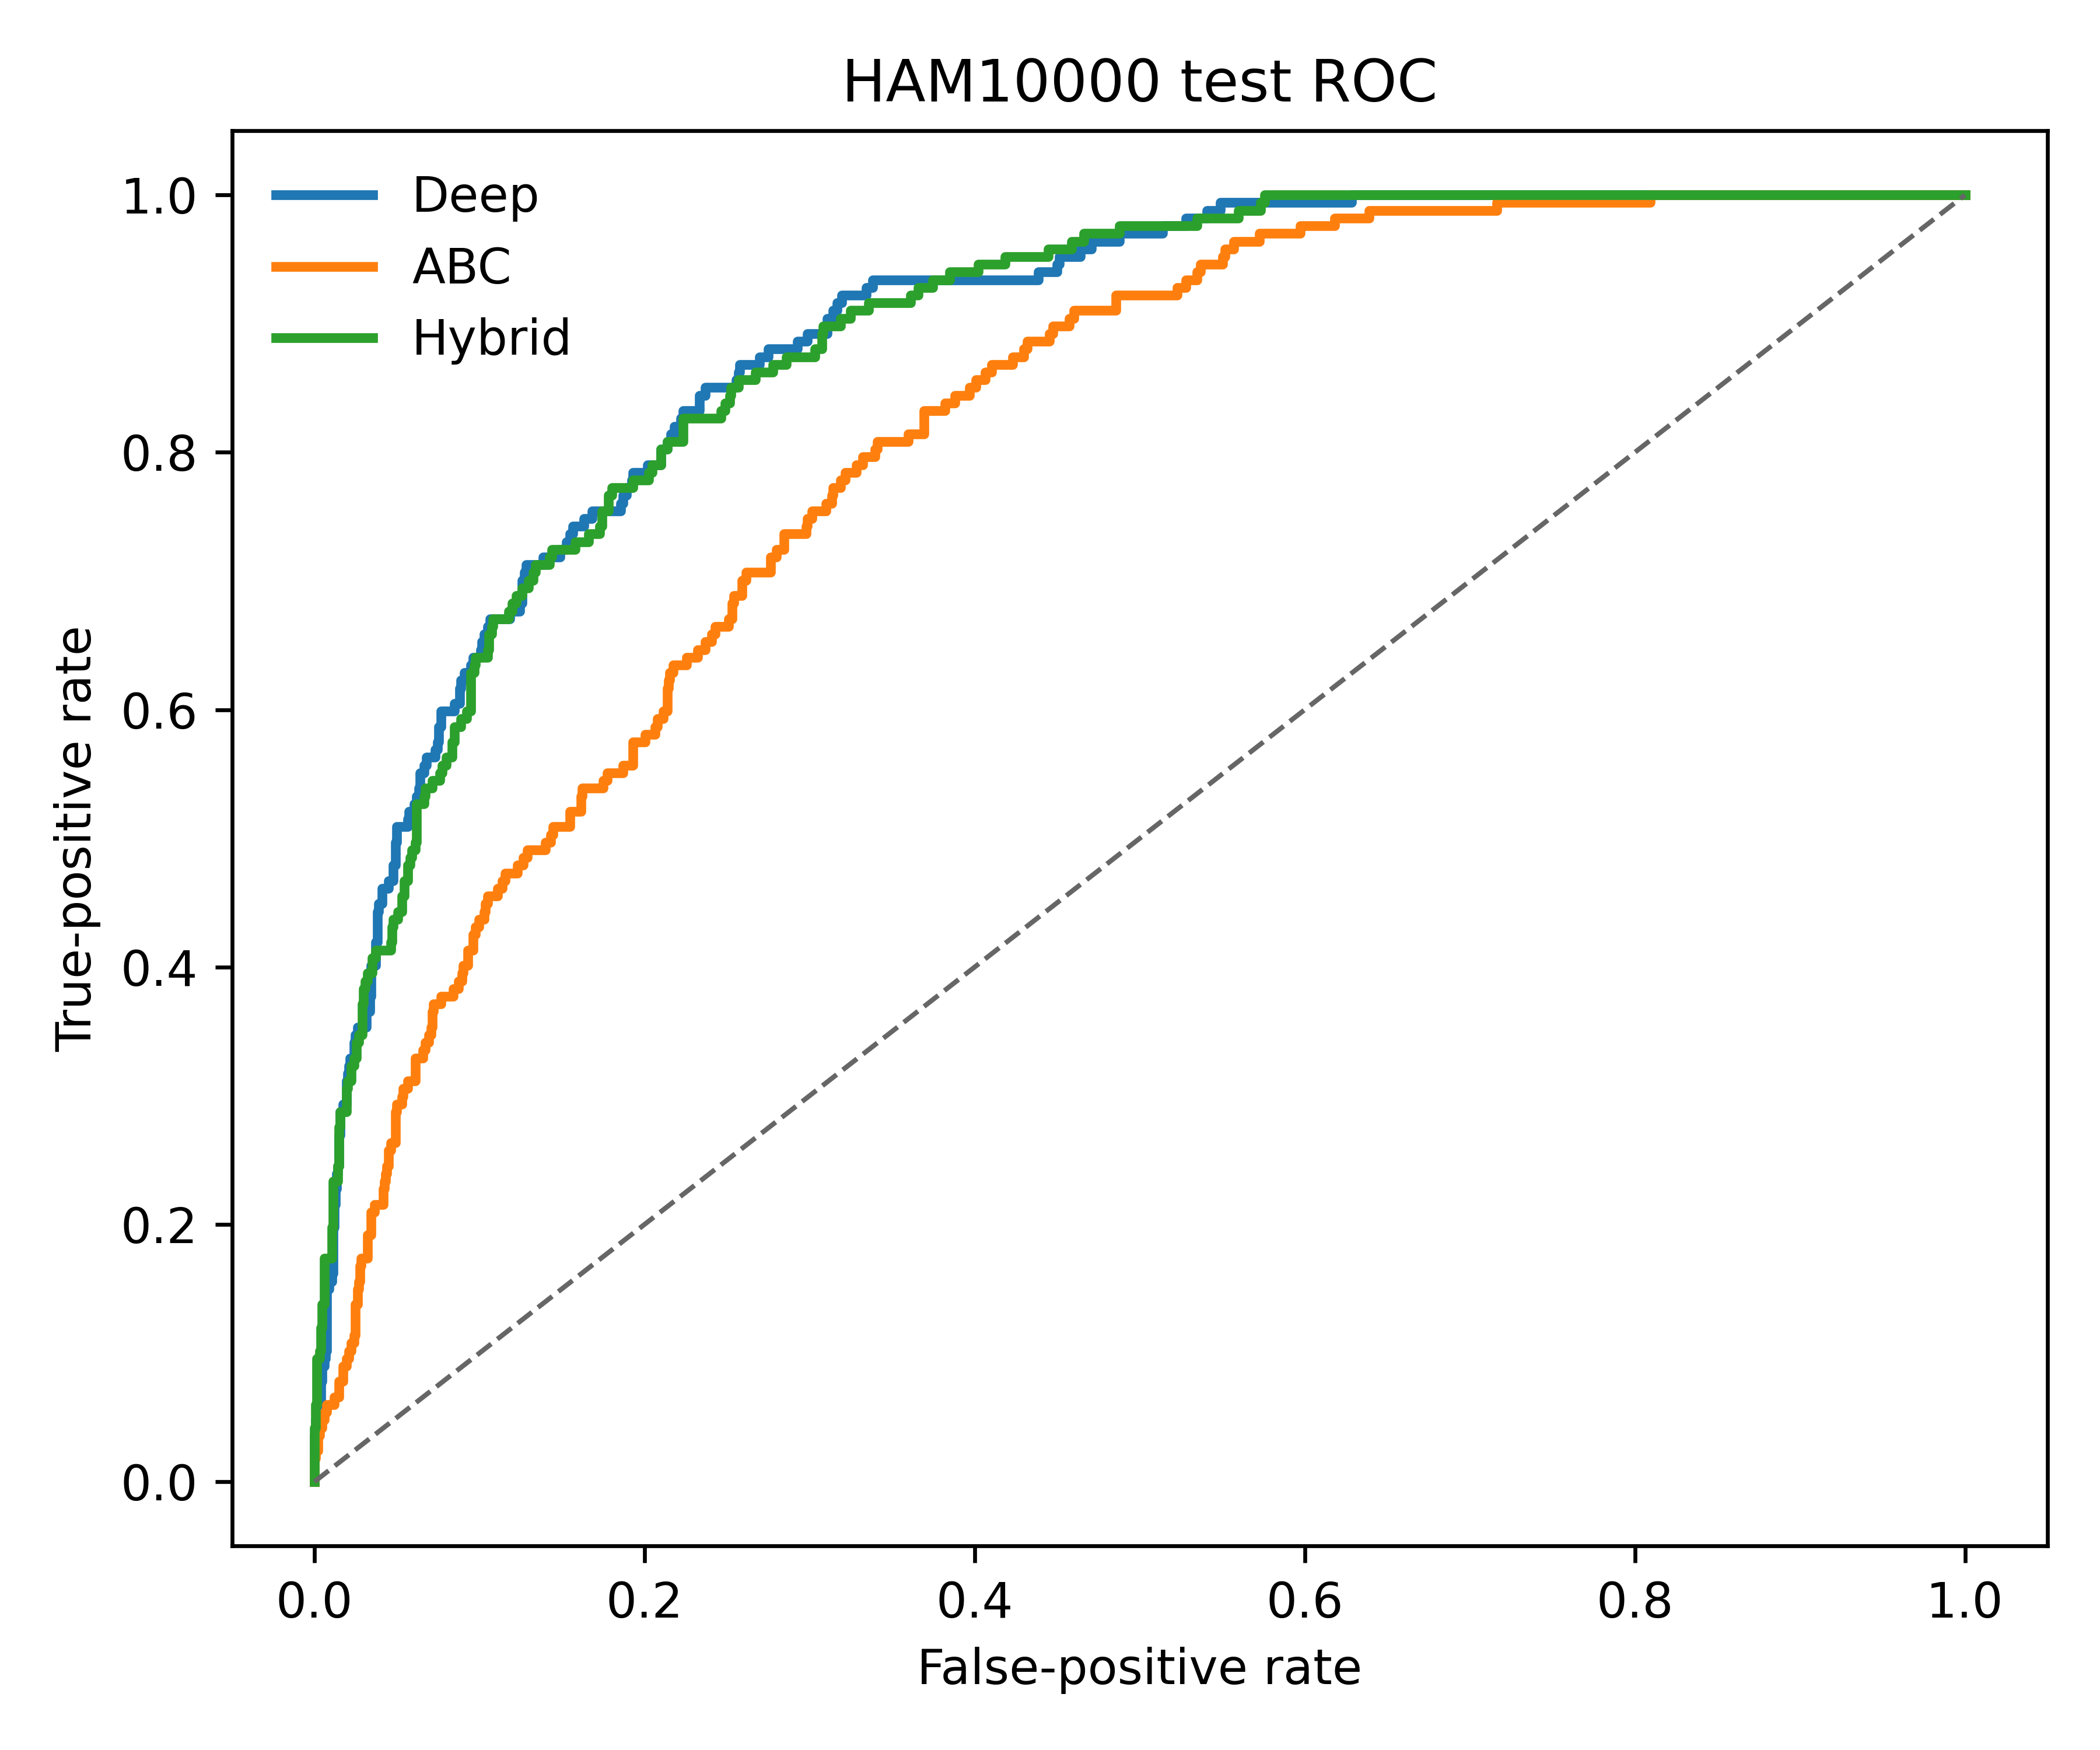
\includegraphics[width=\textwidth]{fig_curves_internal_roc.png}
\caption{ROC.}
\end{subfigure}
\begin{subfigure}[t]{0.32\textwidth}
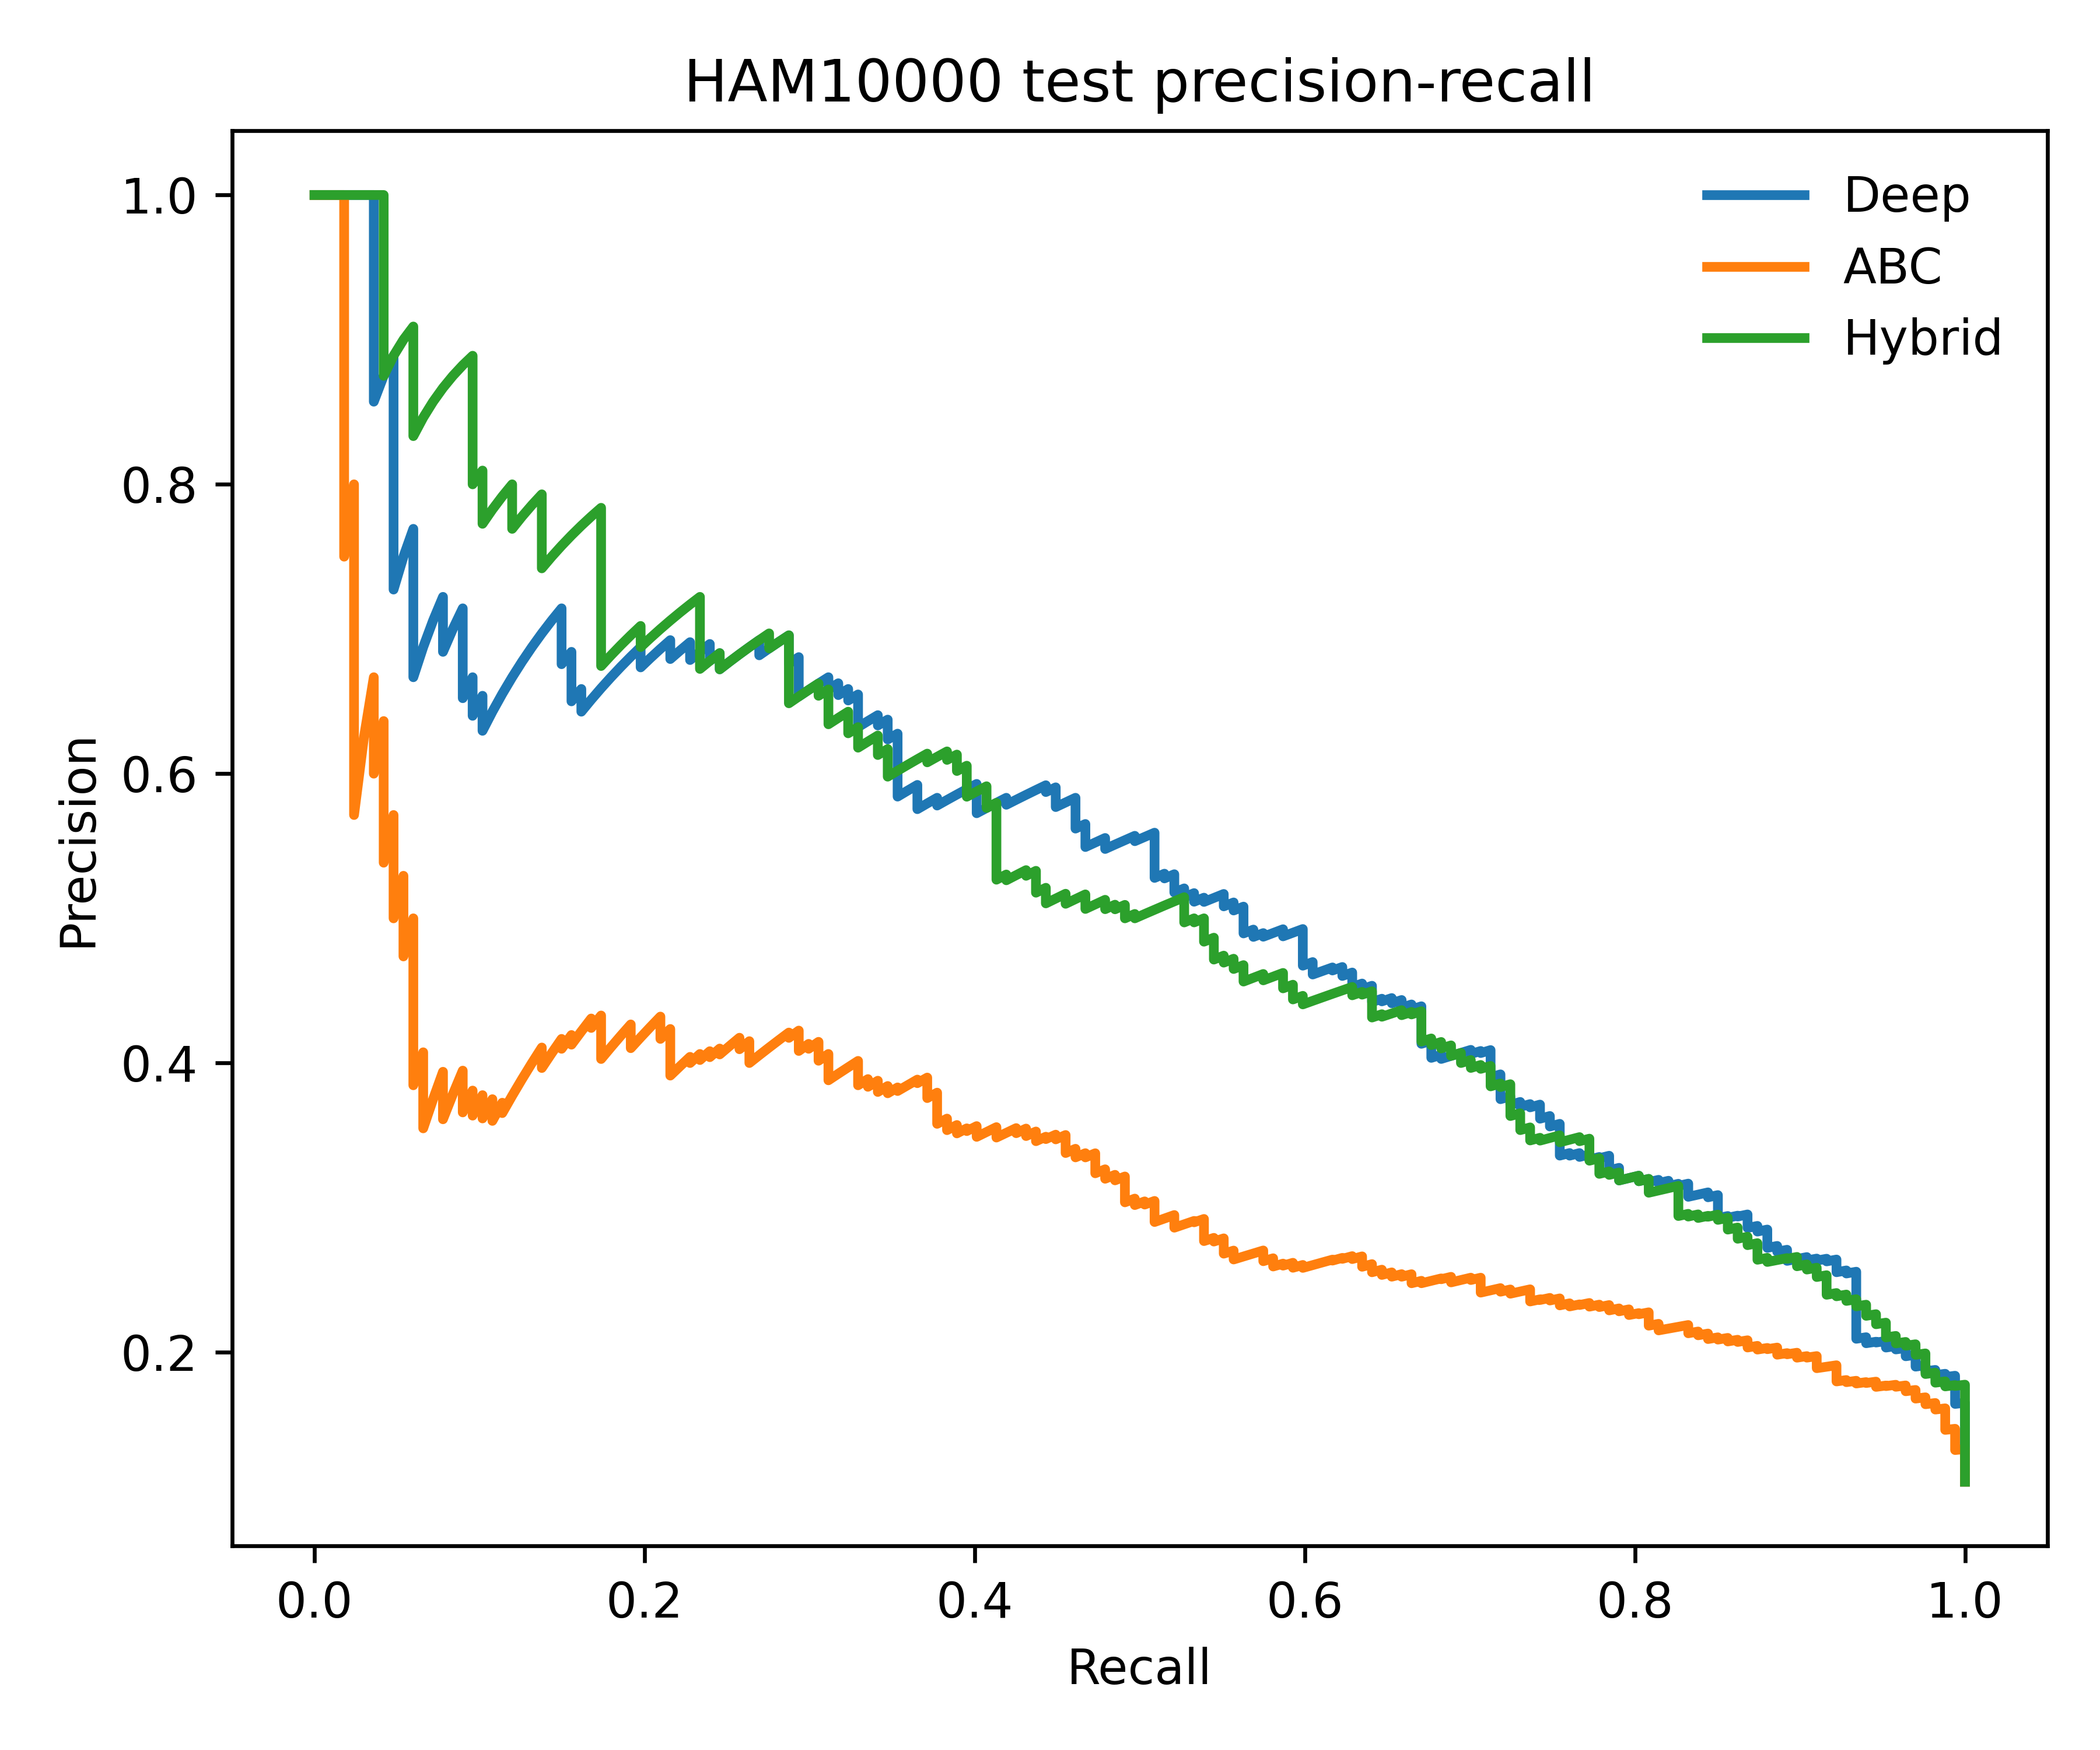
\includegraphics[width=\textwidth]{fig_curves_internal_pr.png}
\caption{Precision-recall.}
\end{subfigure}
\begin{subfigure}[t]{0.32\textwidth}
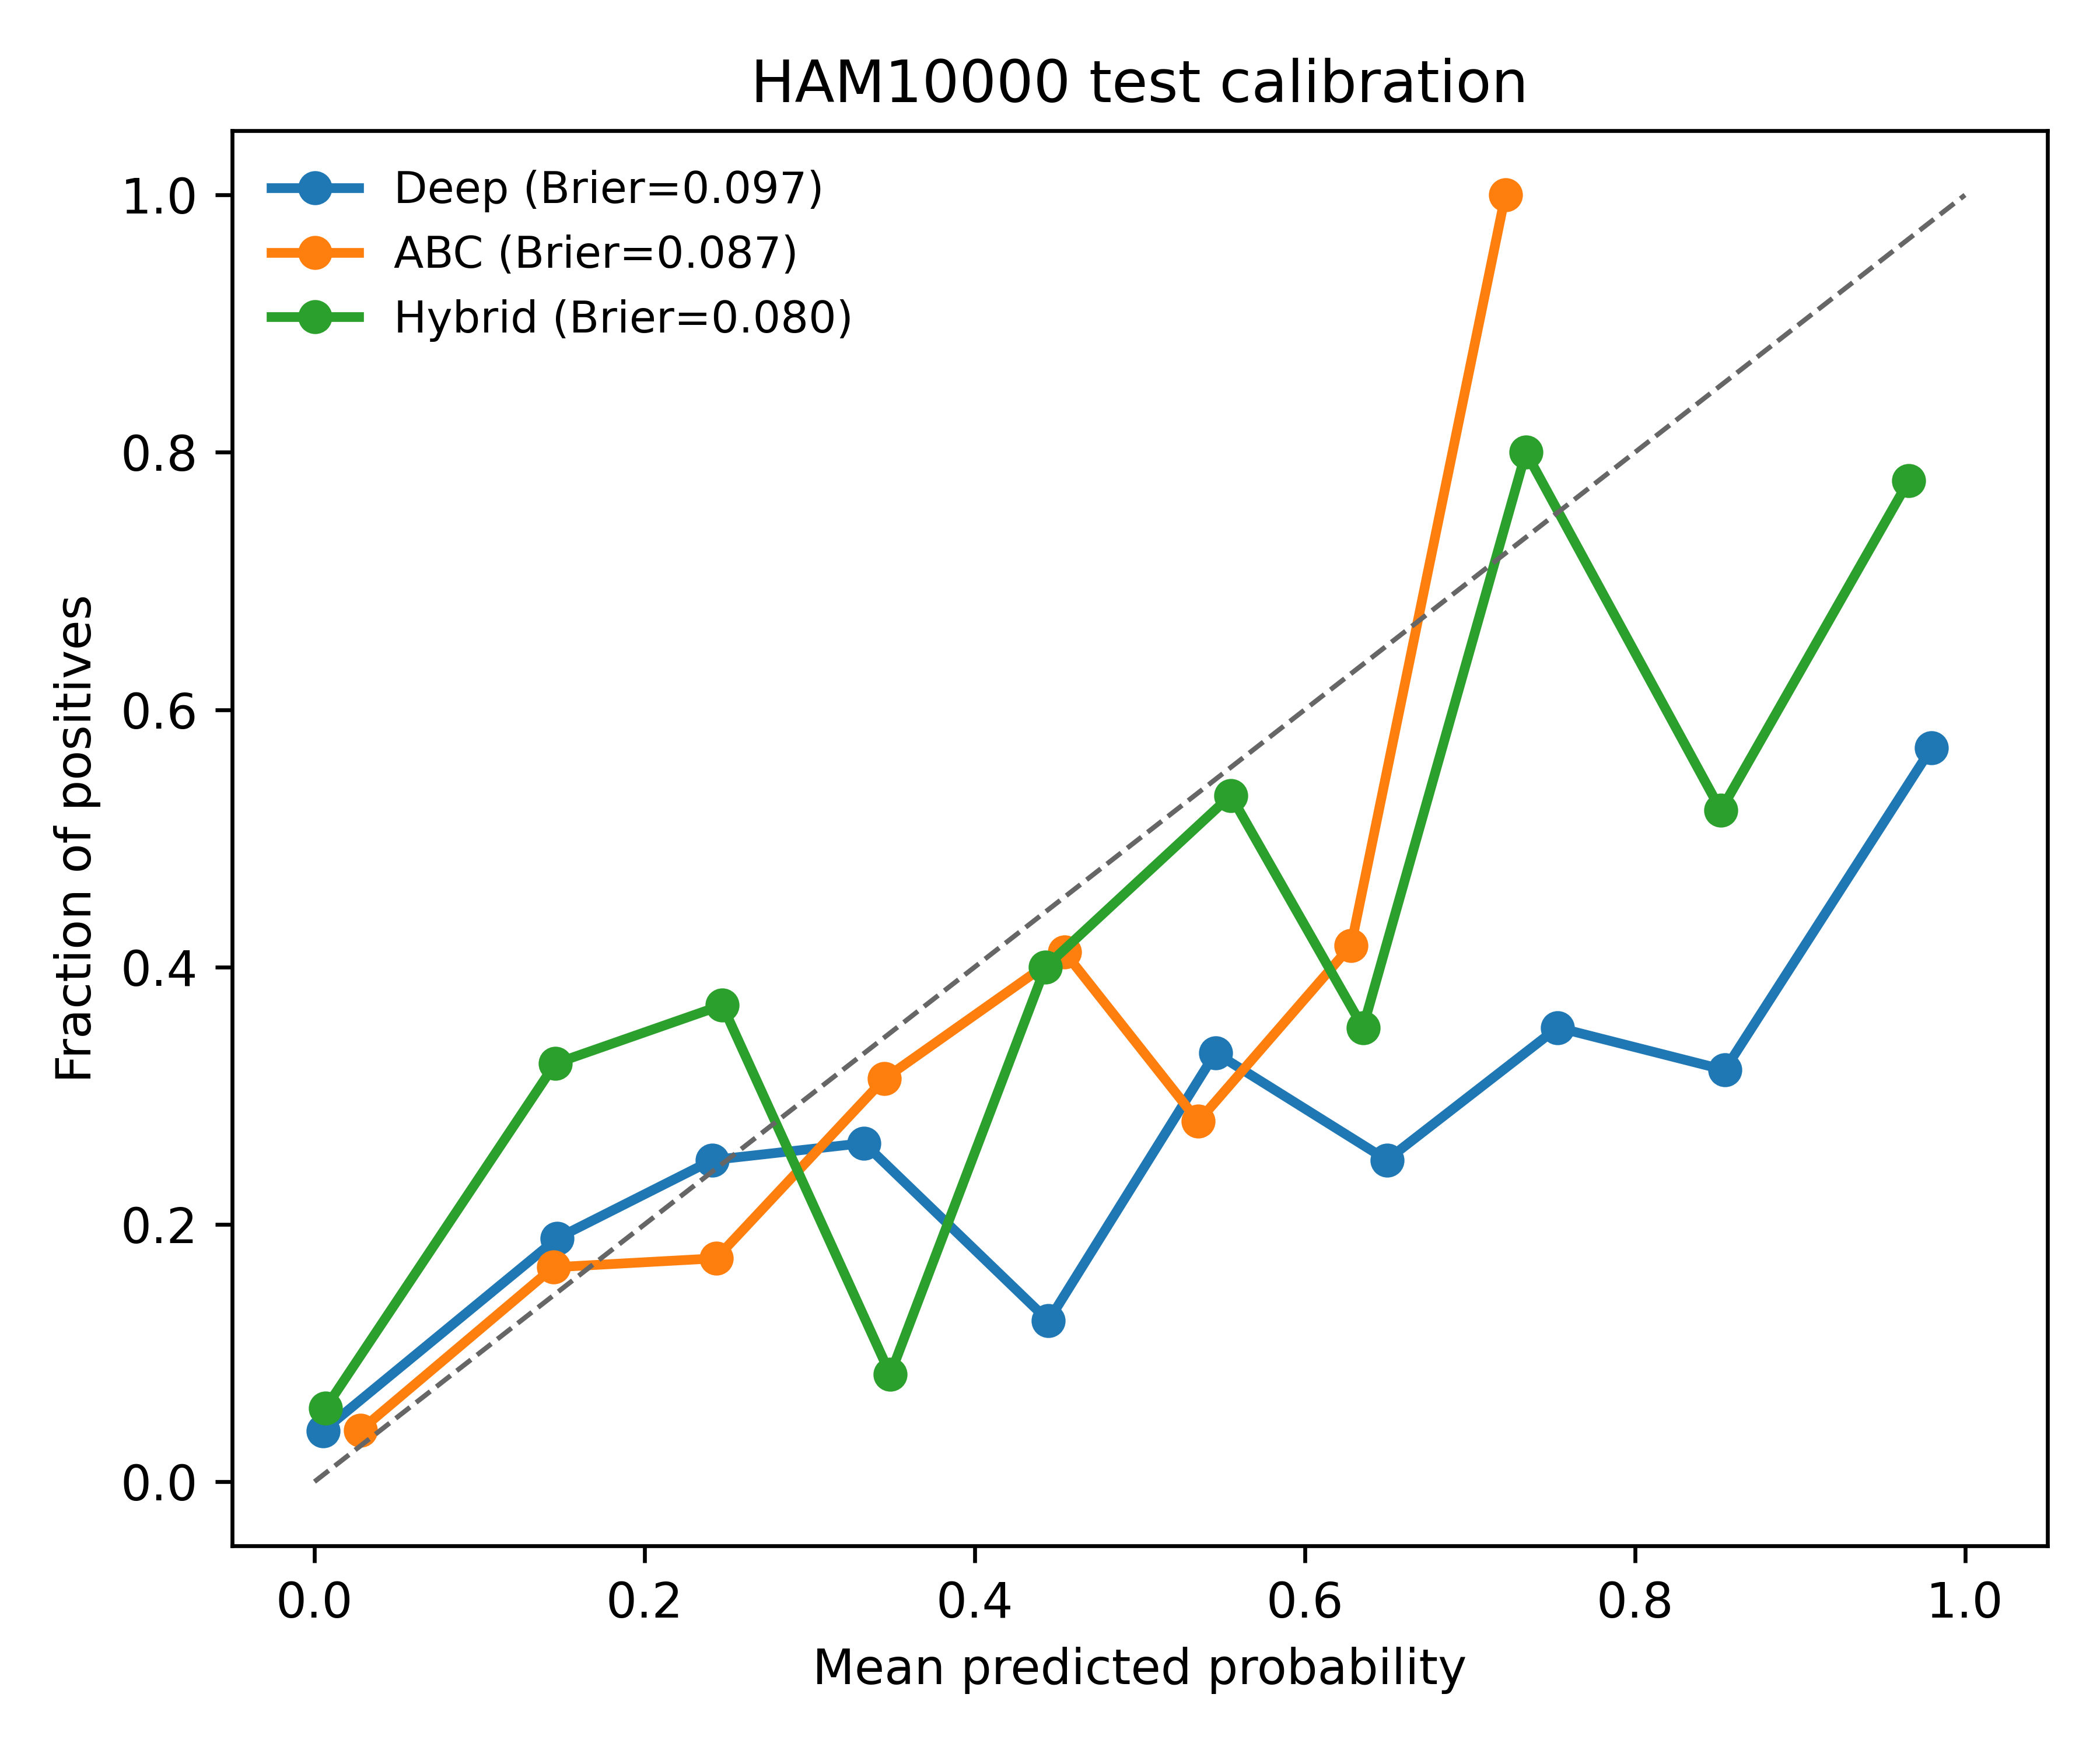
\includegraphics[width=\textwidth]{fig_curves_internal_calibration.png}
\caption{Calibration.}
\end{subfigure}
\caption{Primary HAM10000 lesion-level test curves for all three model families.}
\label{fig:curves_internal}
\end{figure}

\subsection{Secondary ISIC Task 3-label evaluation}

The secondary Task 3-label analysis used the same image corpus and must not be interpreted as independent validation. Within that constraint, all models showed higher apparent discrimination on the full 10,015-image label set than on the held-out HAM10000 test split (Table~\ref{tab:secondary_performance}). This result is expected because the analysis reuses the same public image corpus rather than testing transportability to a non-overlapping cohort.

\begin{table}[htbp]
\centering
\caption{Secondary ISIC 2018 Task 3-label evaluation on the overlapping HAM10000/ISIC image corpus (threshold = 0.5).}
\label{tab:secondary_performance}
\resizebox{\linewidth}{!}{%
\begin{tabular}{lrrrrrrr}
\toprule
Model & AUC & PR-AUC & Brier & F1 & Sens & Spec & Acc \\
\midrule
ABC (XGB) & 0.915 & 0.633 & 0.065 & 0.377 & 0.246 & 0.993 & 0.910 \\
Deep (EffB0) & 0.979 & 0.916 & 0.032 & 0.834 & 0.884 & 0.970 & 0.961 \\
Hybrid (ABC+Emb) & 0.982 & 0.935 & 0.022 & 0.872 & 0.820 & 0.992 & 0.973 \\
\bottomrule
\end{tabular}%
}
\end{table}

\begin{figure}[H]
\centering
\begin{subfigure}[t]{0.32\textwidth}
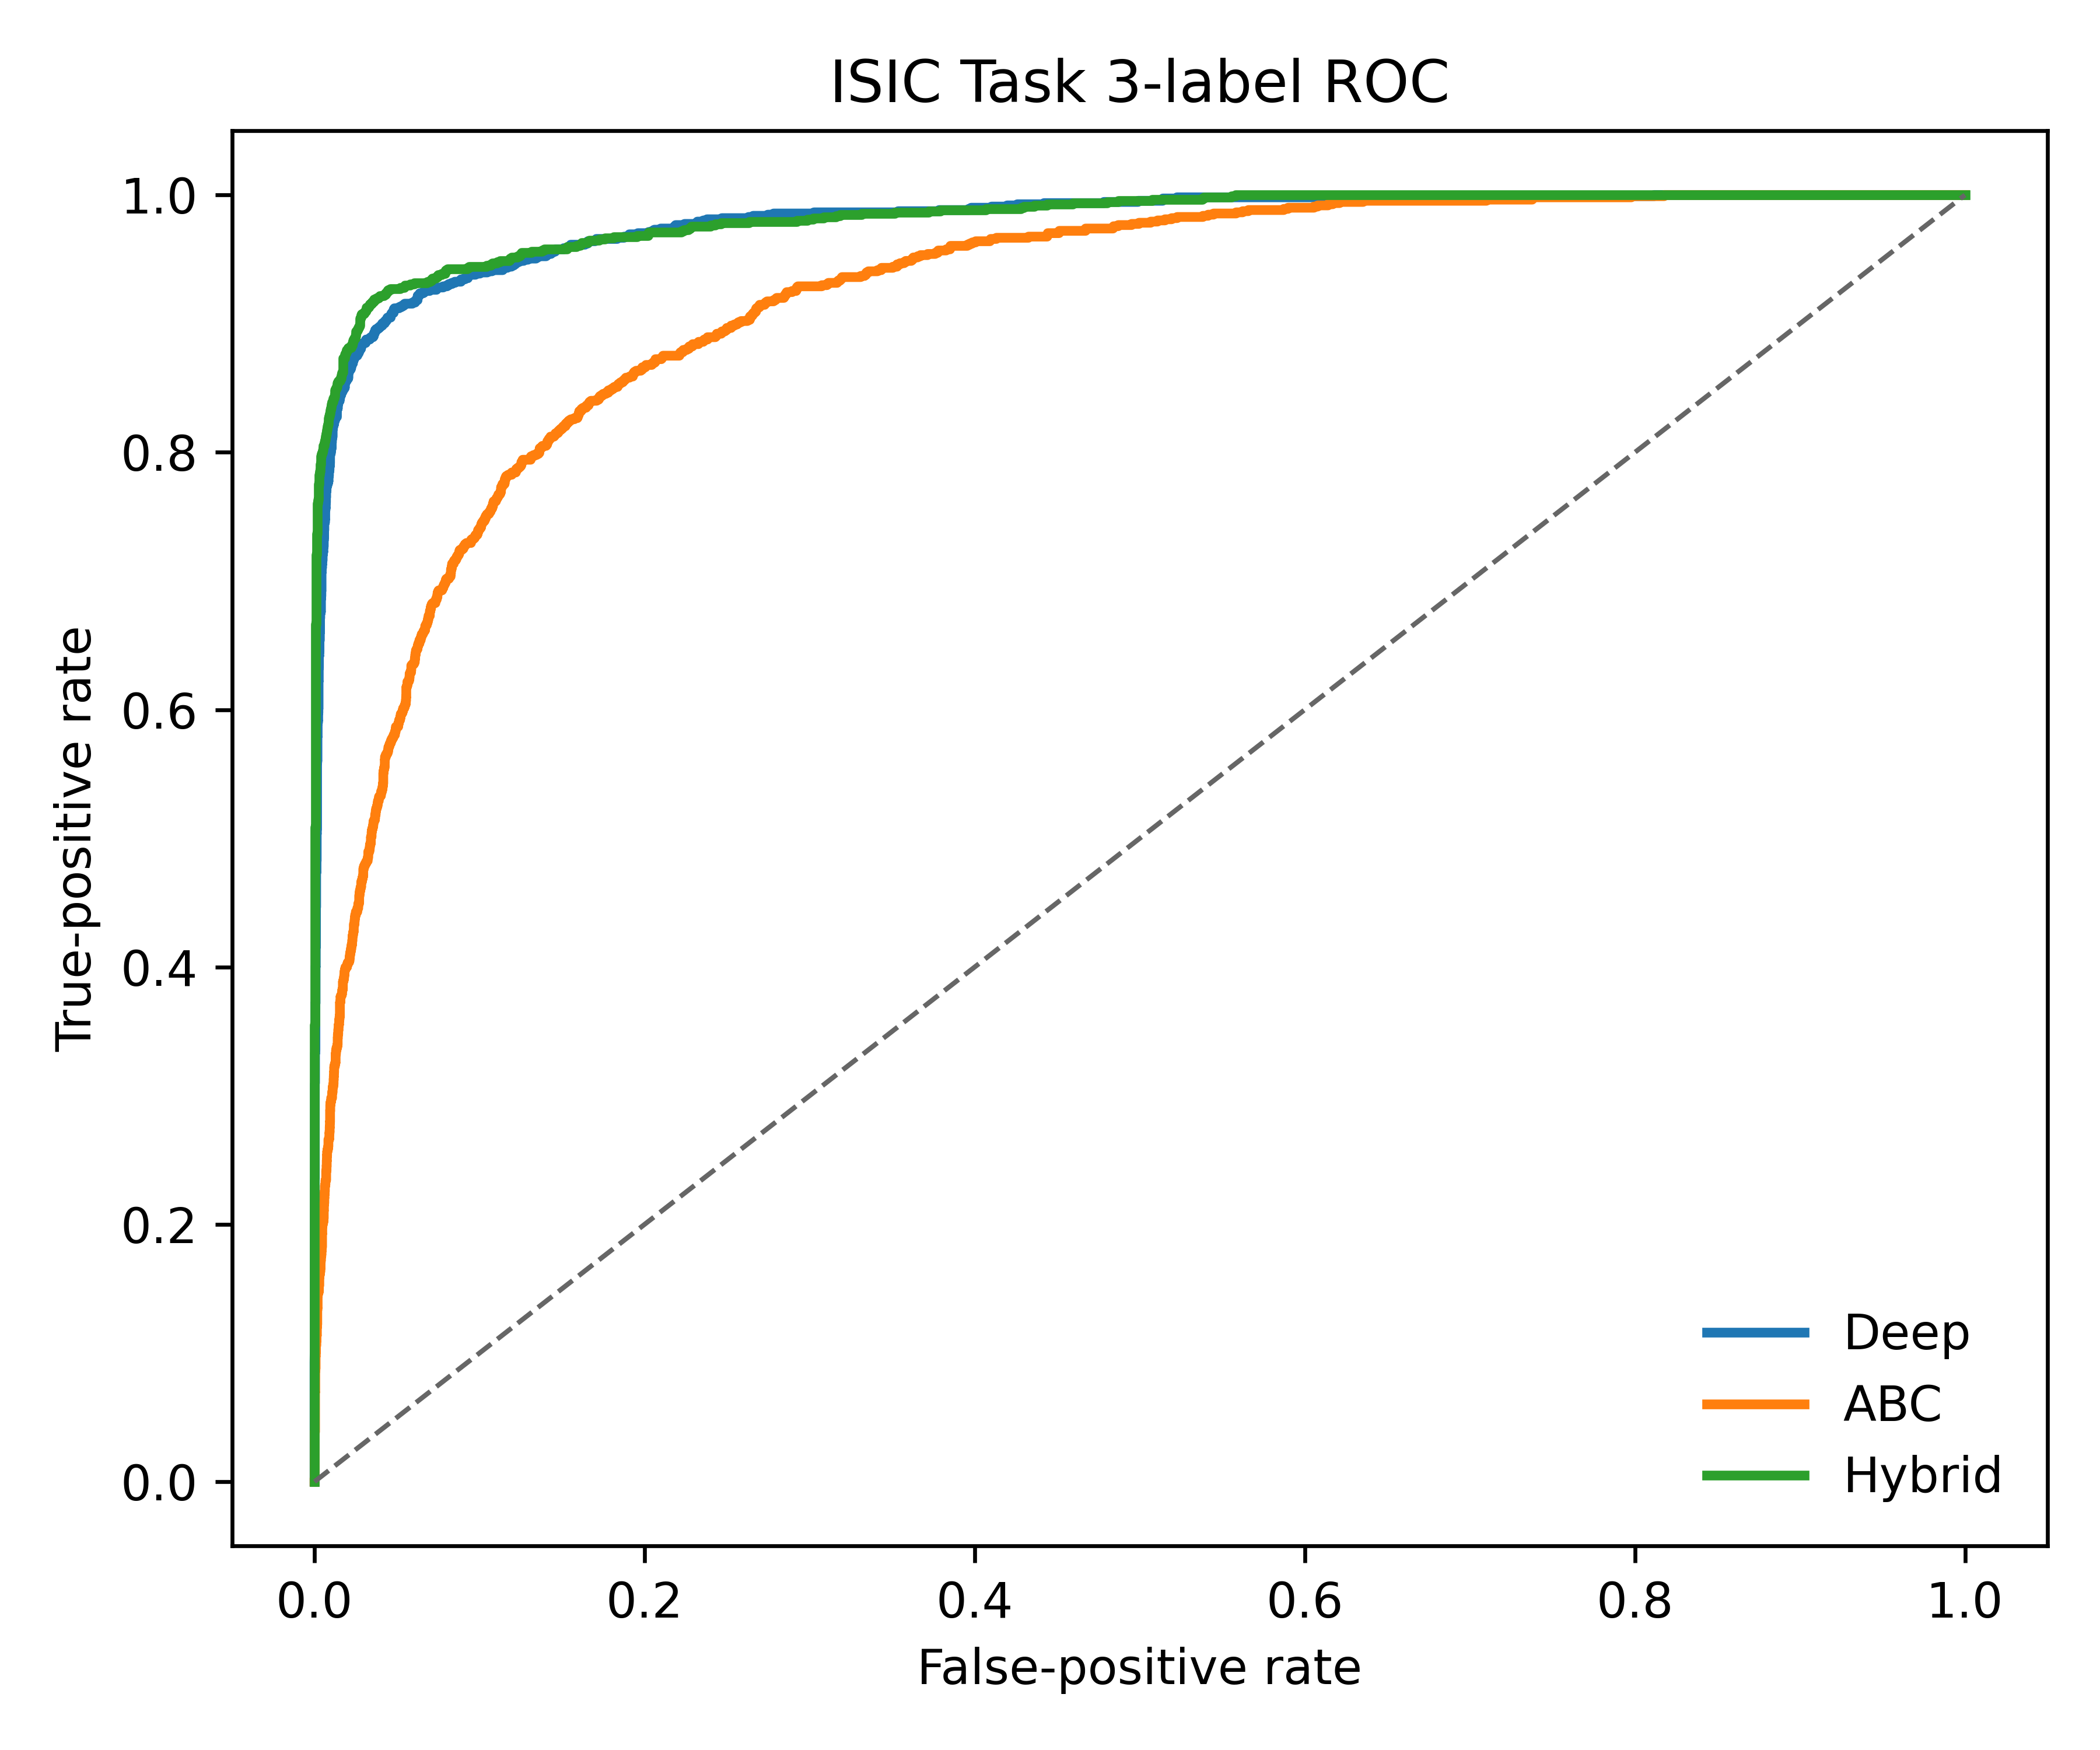
\includegraphics[width=\textwidth]{fig_curves_secondary_roc.png}
\caption{ROC.}
\end{subfigure}
\begin{subfigure}[t]{0.32\textwidth}
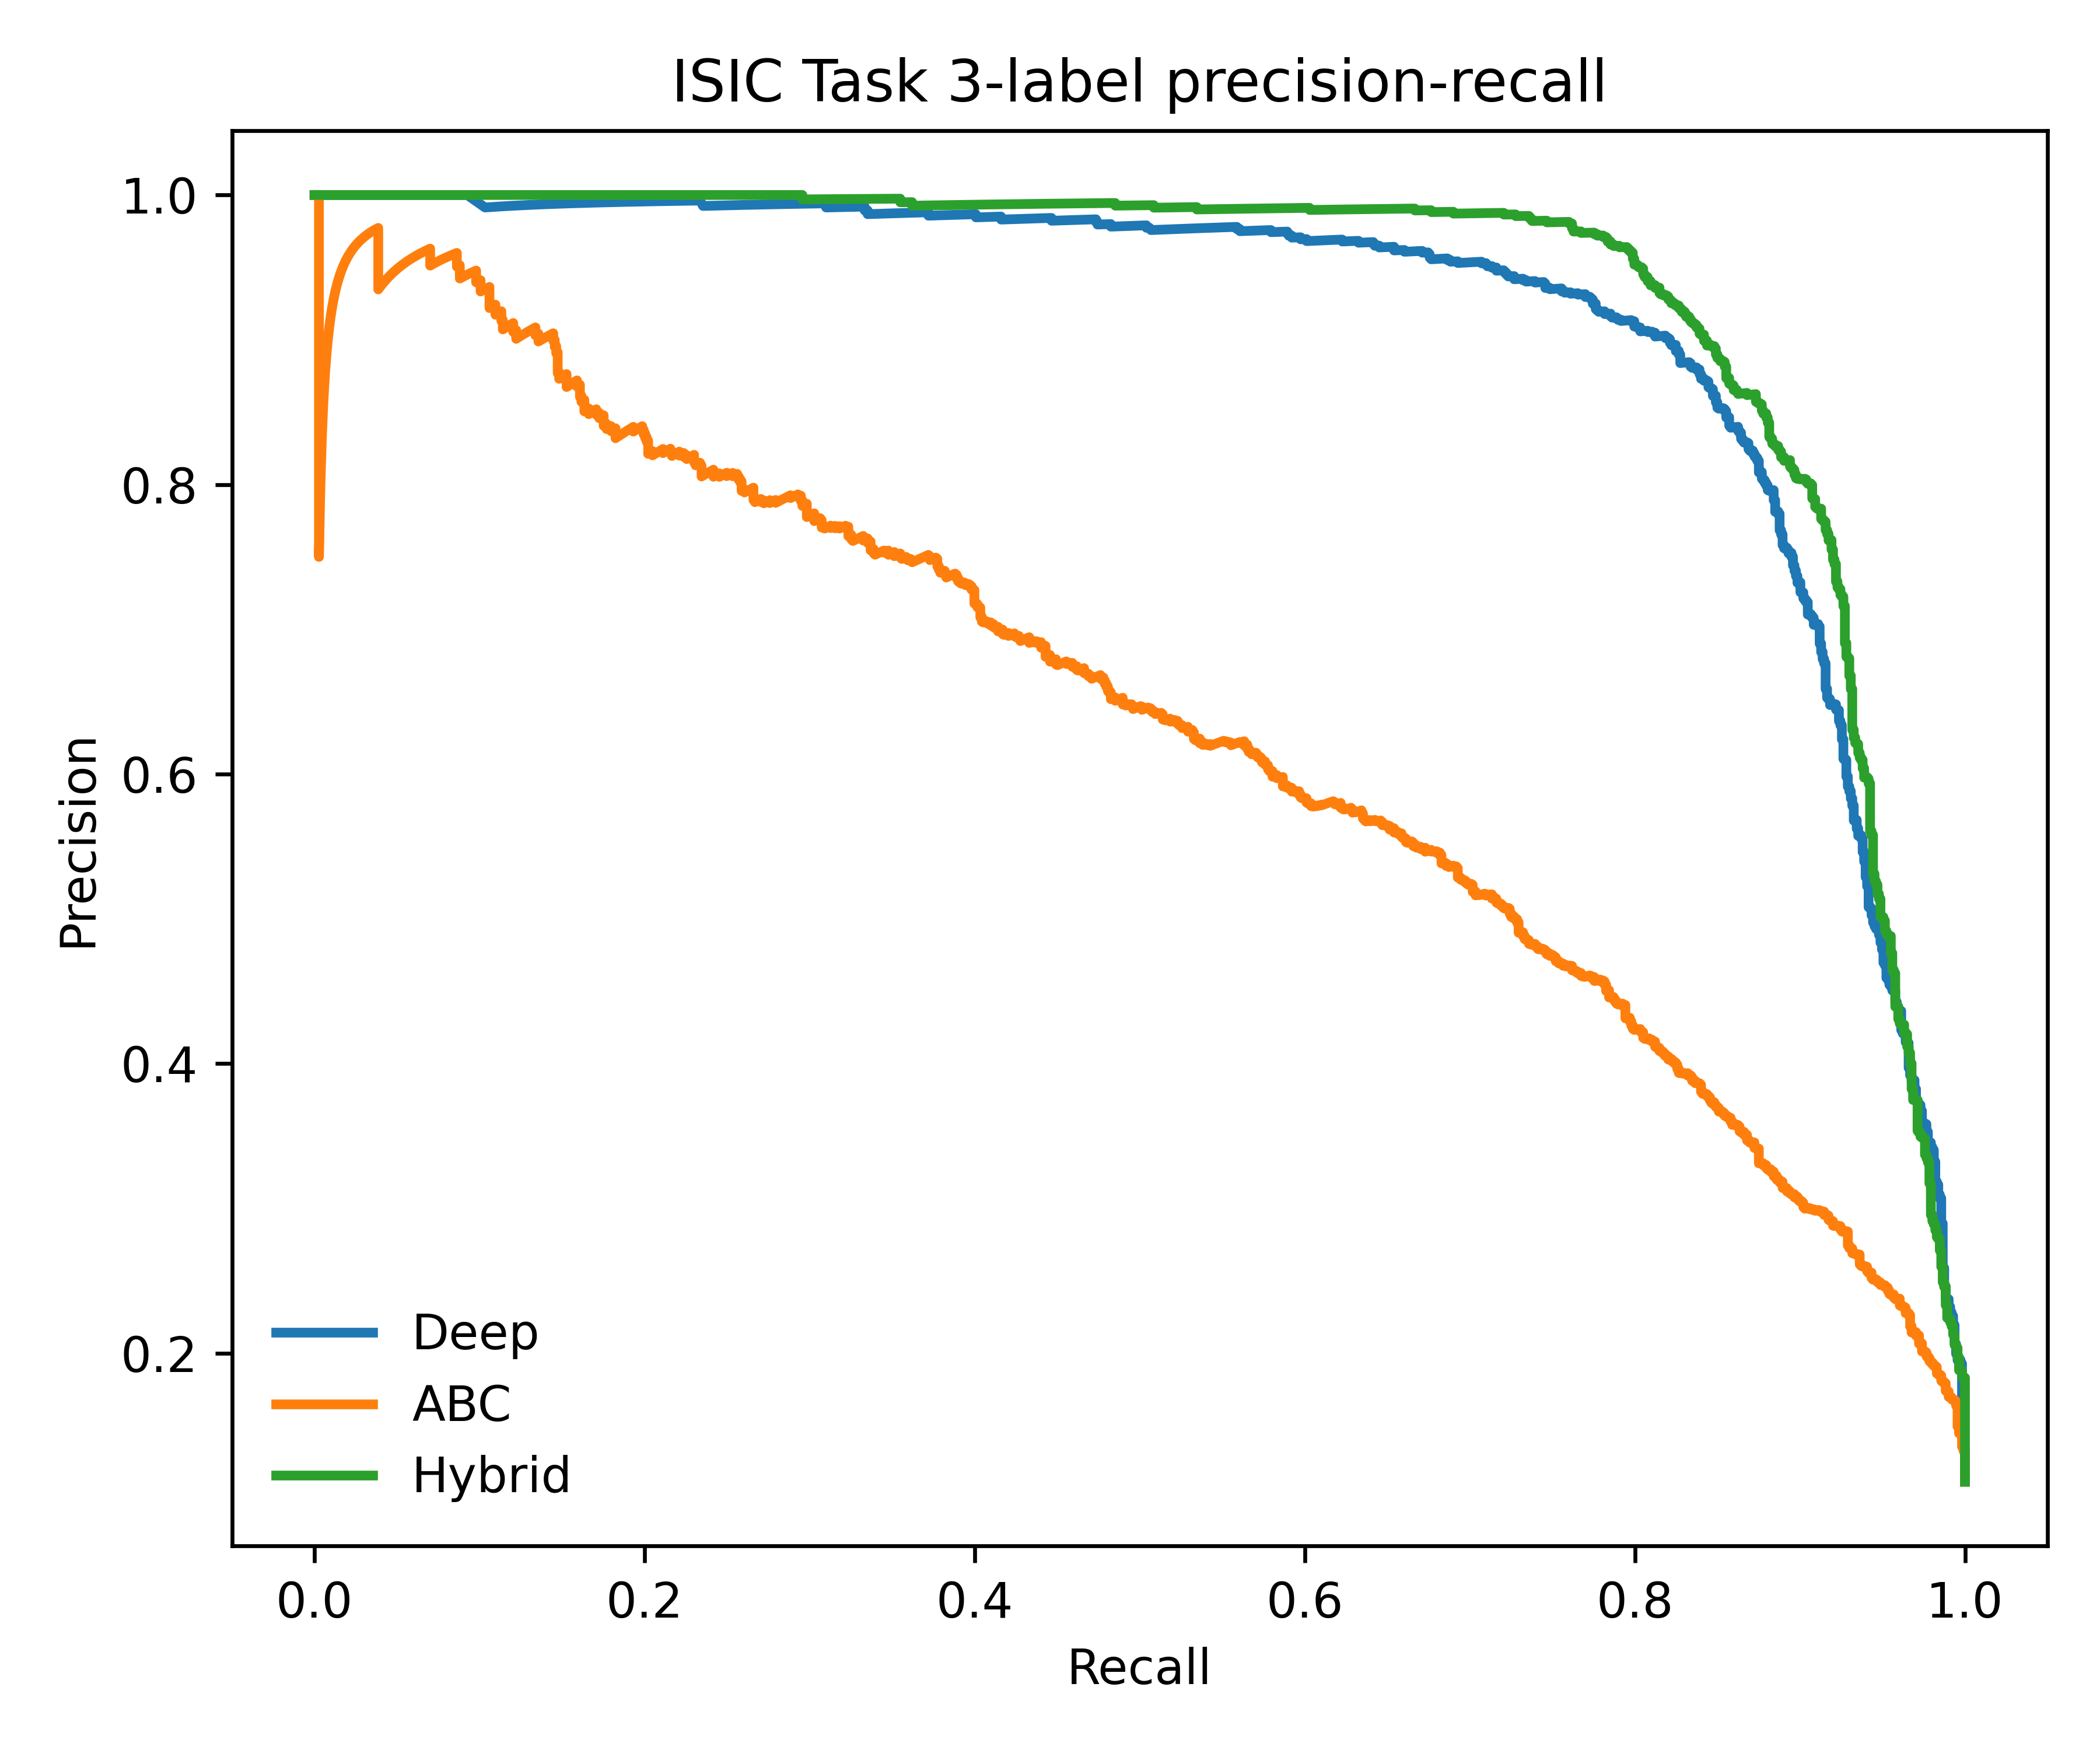
\includegraphics[width=\textwidth]{fig_curves_secondary_pr.png}
\caption{Precision-recall.}
\end{subfigure}
\begin{subfigure}[t]{0.32\textwidth}
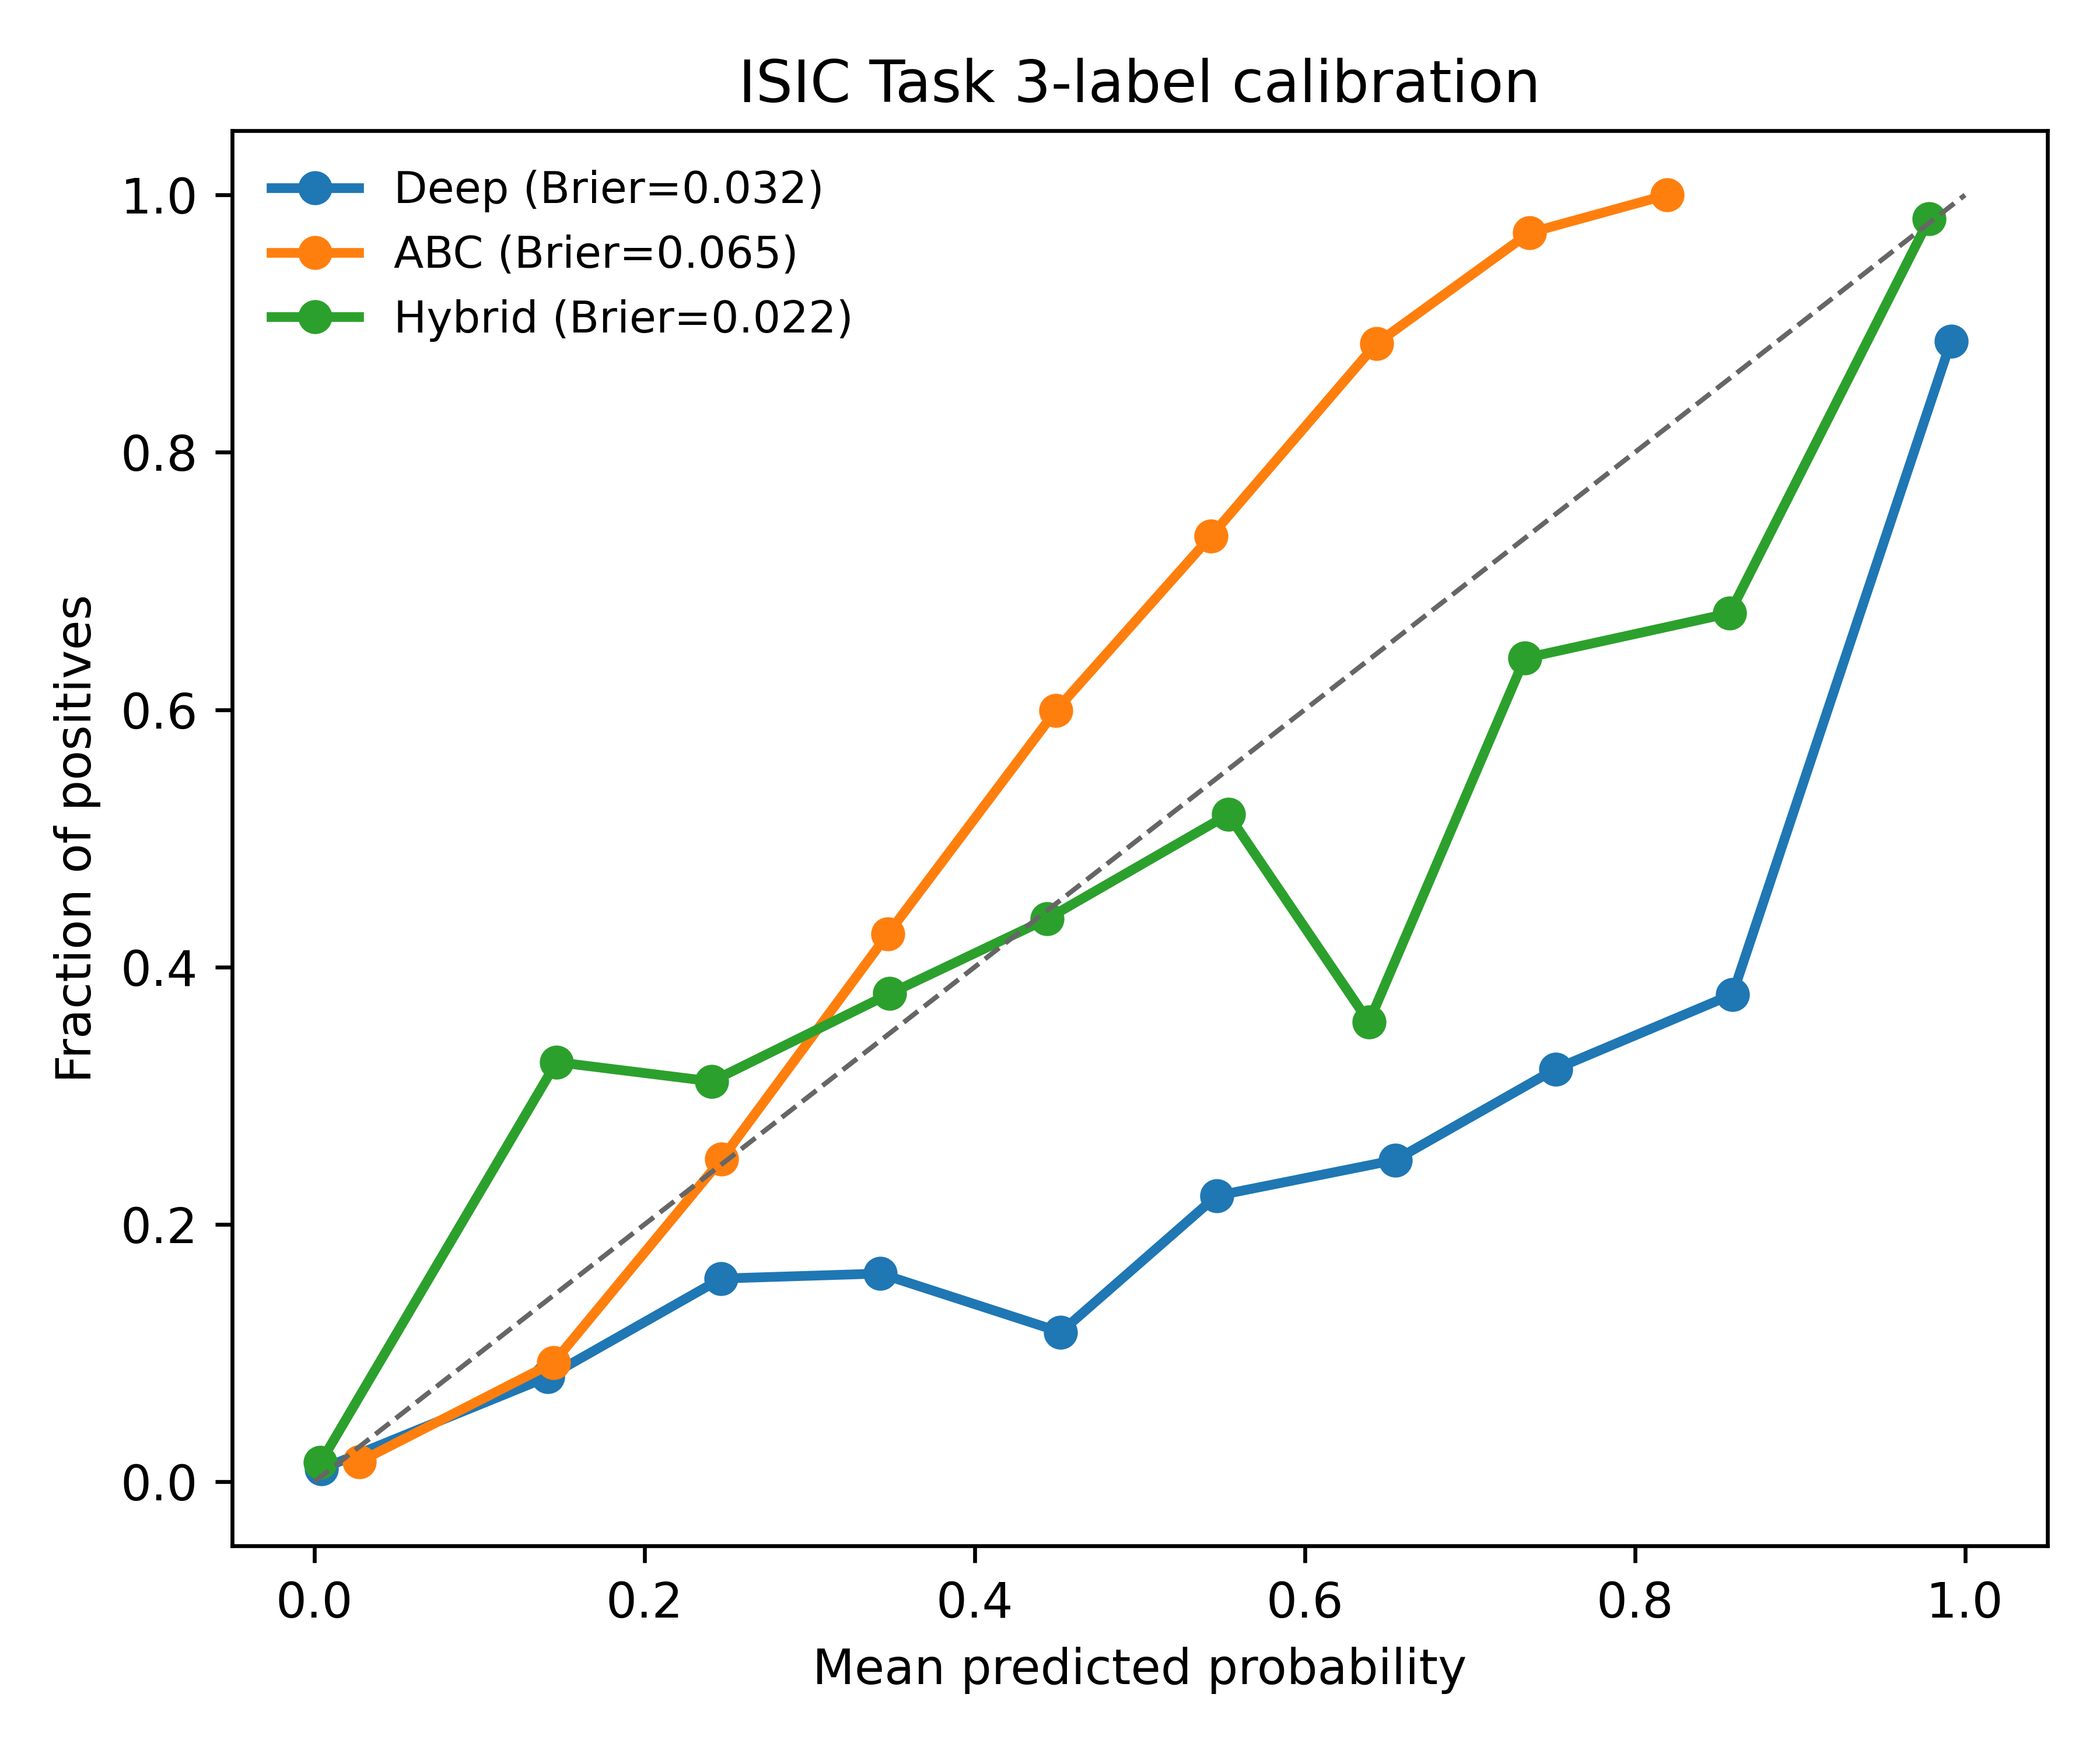
\includegraphics[width=\textwidth]{fig_curves_secondary_calibration.png}
\caption{Calibration.}
\end{subfigure}
\caption{Secondary ISIC Task 3-label curves. These curves are reported as within-corpus label evaluation only because image overlap with HAM10000 is complete.}
\label{fig:curves_secondary}
\end{figure}

\subsection{Independent BCN20000 External Validation}

After verifying zero overlap between the HAM10000 training instances and the BCN20000 cohort via exact identifier and perceptual hash auditing, the frozen models were evaluated on the BCN20000 images. No retraining or fine-tuning was performed.

As shown in Table~\ref{tab:bcn20000_performance}, the models generalized robustly to the external cohort despite a rigorous domain shift. The Deep EfficientNet-B0 baseline achieved an AUC of 0.713 and a Brier score of 0.190. The Hybrid model achieved an AUC of 0.761 with a Brier score of 0.189. The ABC-only model yielded an AUC of 0.692. 

\begin{table}[htbp]
\centering
\caption{Independent BCN20000 external validation performance (threshold = 0.5) after zero-overlap audit.}
\label{tab:bcn20000_performance}
\resizebox{\linewidth}{!}{%
\begin{tabular}{lrrrrrrr}
\toprule
Model & AUC & PR-AUC & Brier & F1 & Sens & Spec & Acc \\
\midrule
ABC (XGB) & 0.692 & 0.379 & 0.186 & 0.027 & 0.014 & 0.998 & 0.772 \\
Deep (EffB0) & 0.713 & 0.472 & 0.190 & 0.337 & 0.232 & 0.957 & 0.790 \\
Hybrid (ABC+Emb) & 0.761 & 0.548 & 0.189 & 0.244 & 0.143 & 0.991 & 0.796 \\
\bottomrule
\end{tabular}%
}
\end{table}

The corresponding threshold-agnostic curves (Figure~\ref{fig:curves_bcn}) and decision-curve analysis (Figure~\ref{fig:dca_bcn}) confirm that the probability estimates remained reasonably calibrated and provided net clinical benefit on the completely independent data.

\begin{figure}[H]
\centering
\begin{subfigure}[t]{0.32\textwidth}
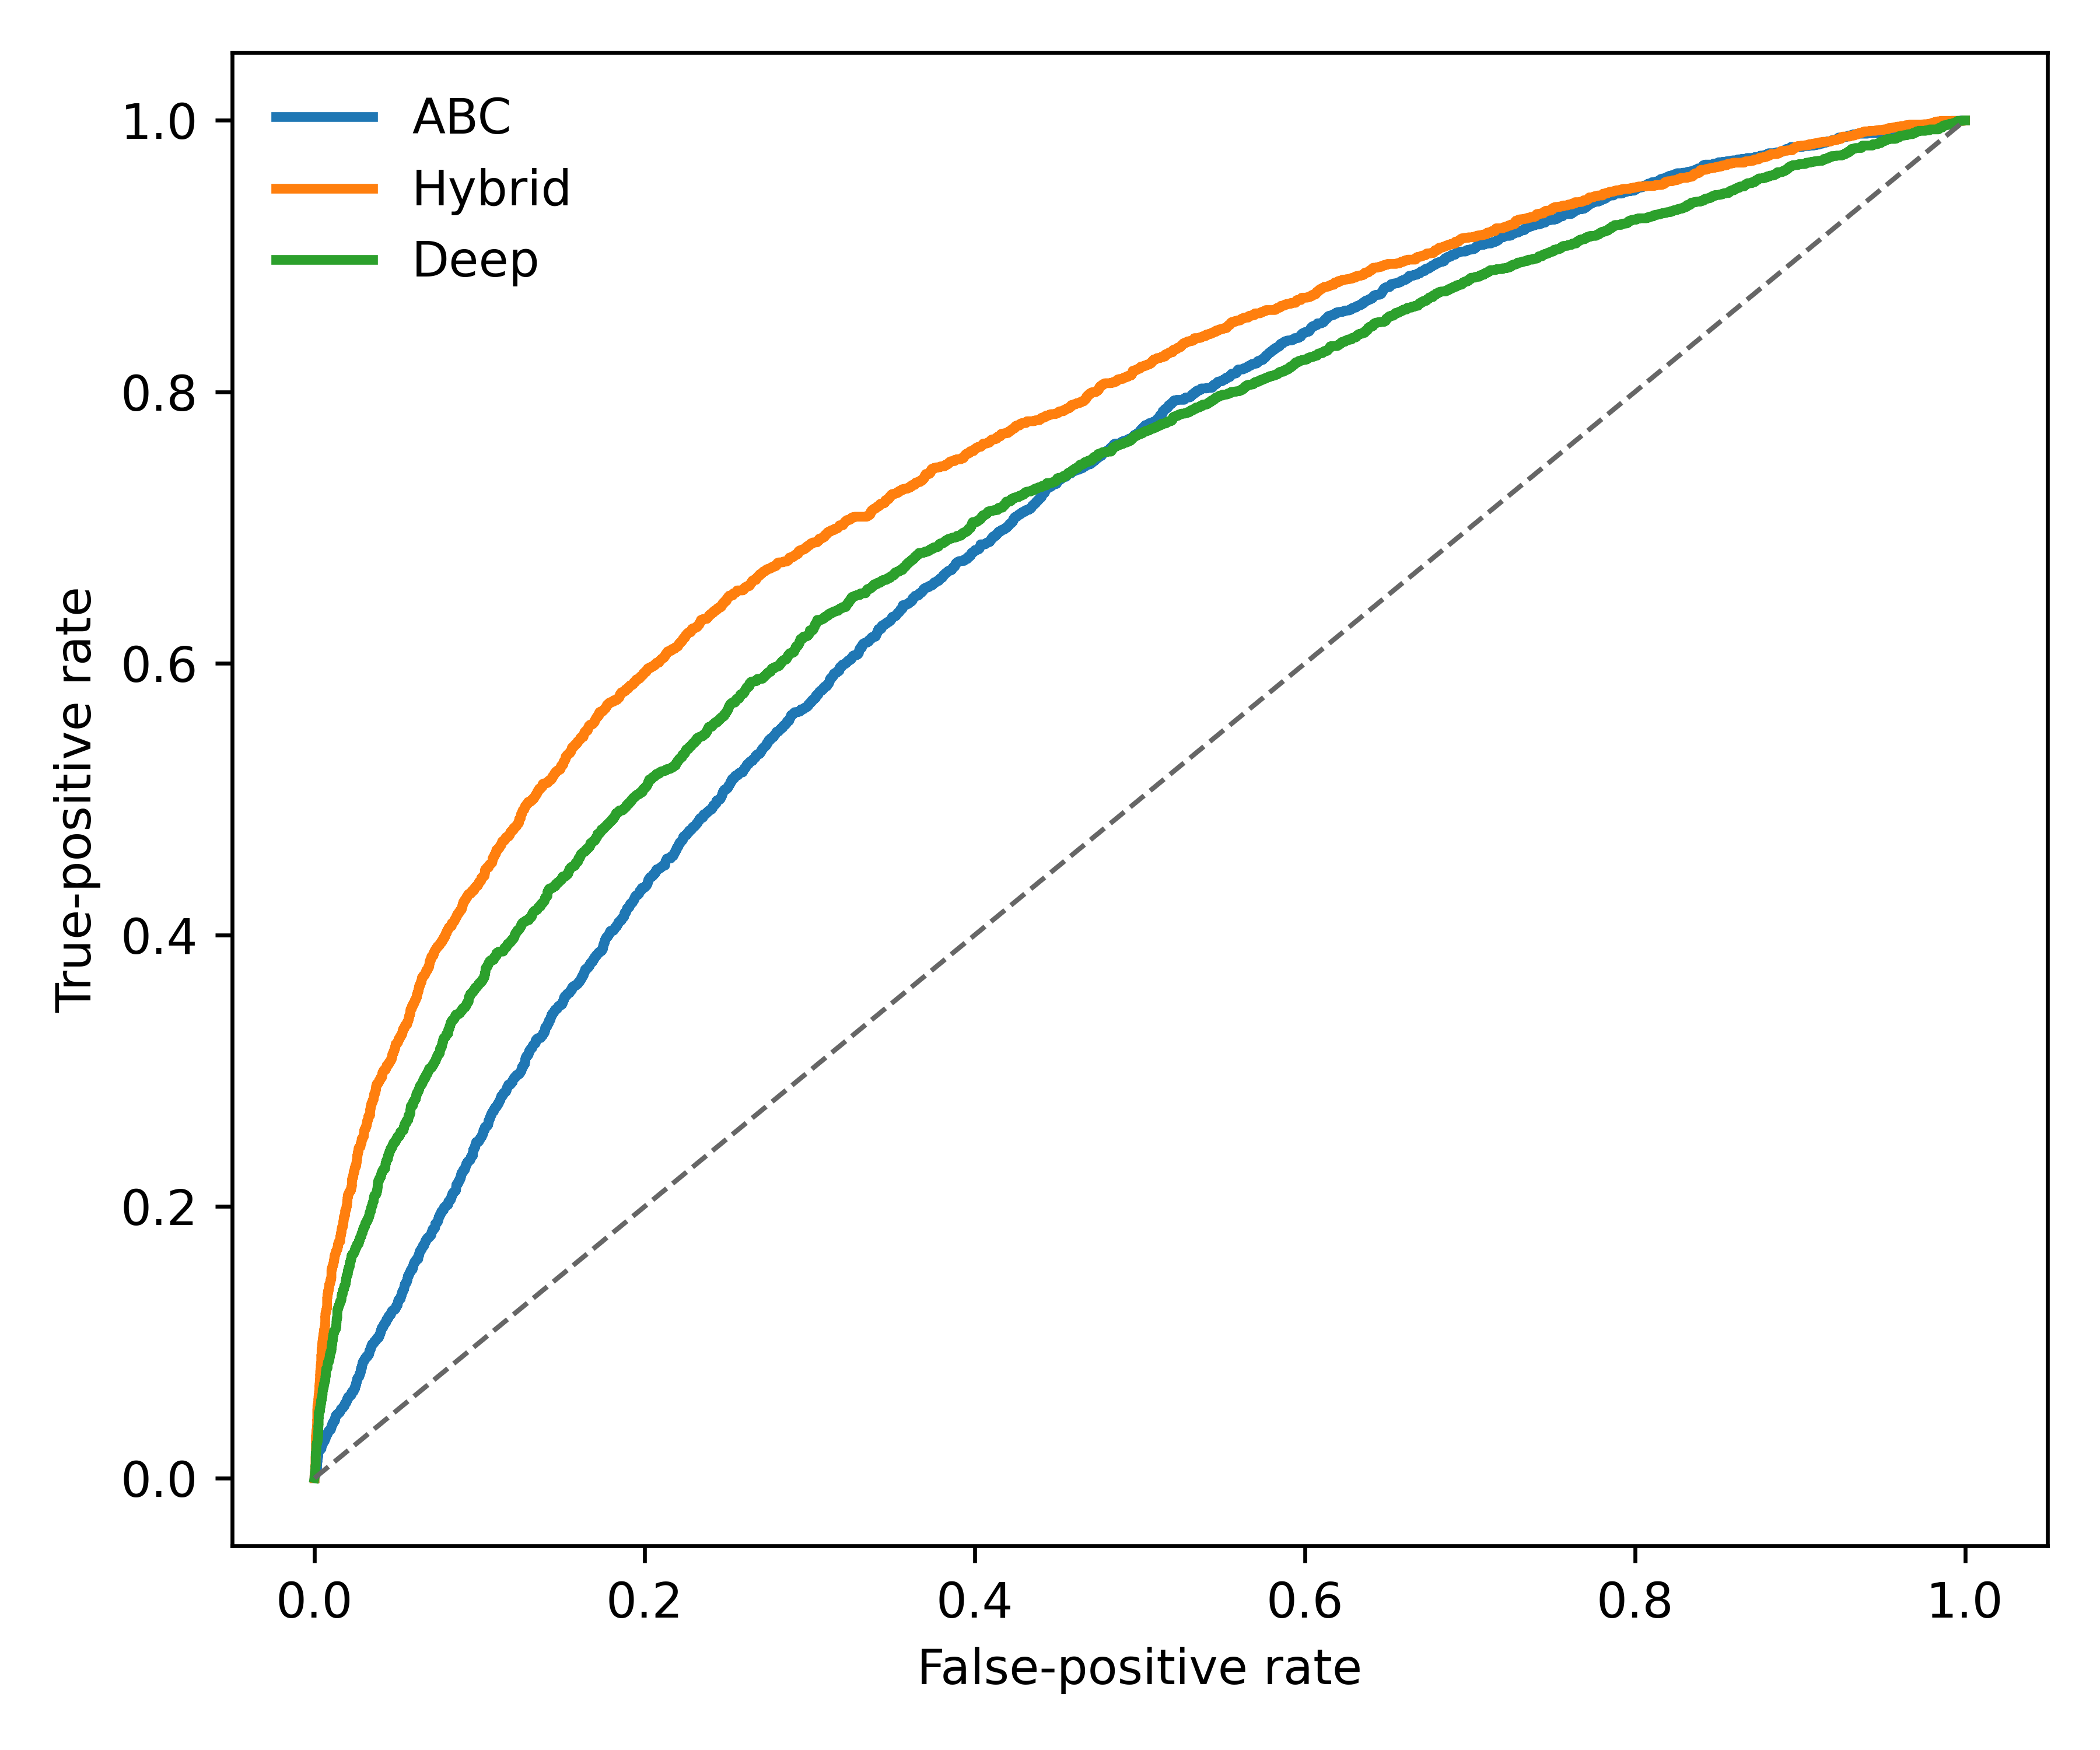
\includegraphics[width=\textwidth]{fig_curves_bcn_roc.png}
\caption{ROC.}
\end{subfigure}
\begin{subfigure}[t]{0.32\textwidth}
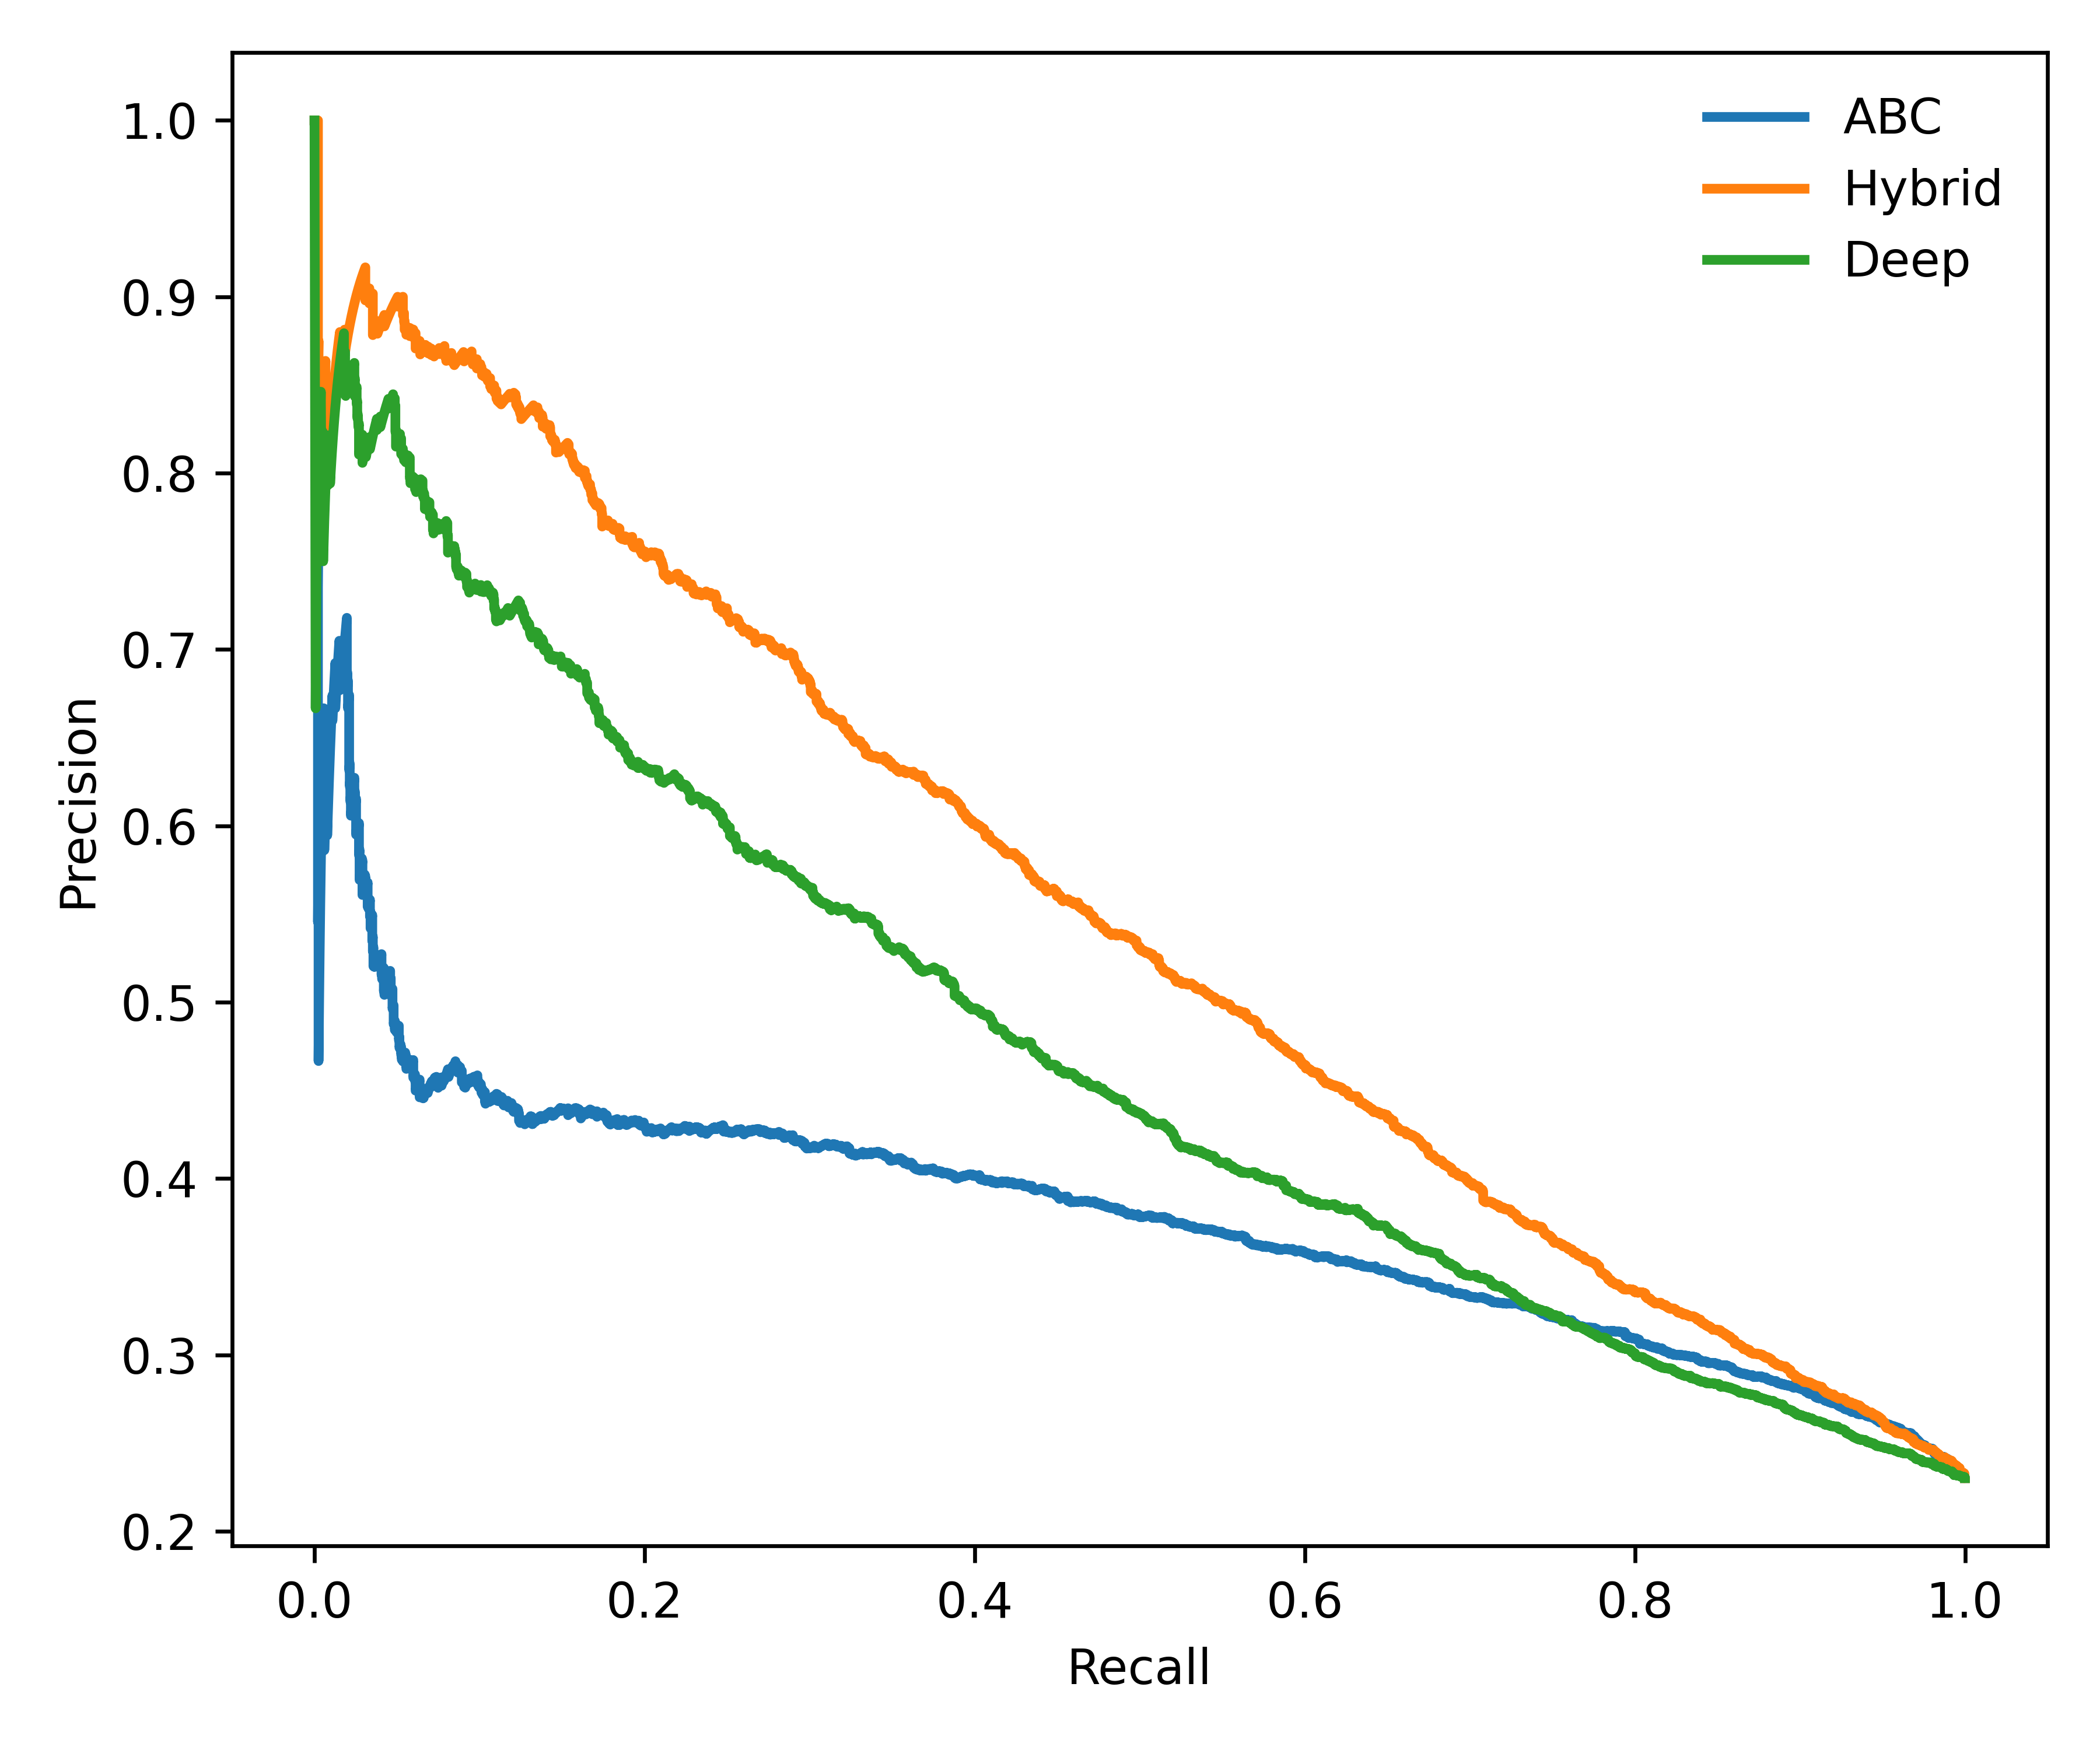
\includegraphics[width=\textwidth]{fig_curves_bcn_pr.png}
\caption{Precision-recall.}
\end{subfigure}
\begin{subfigure}[t]{0.32\textwidth}
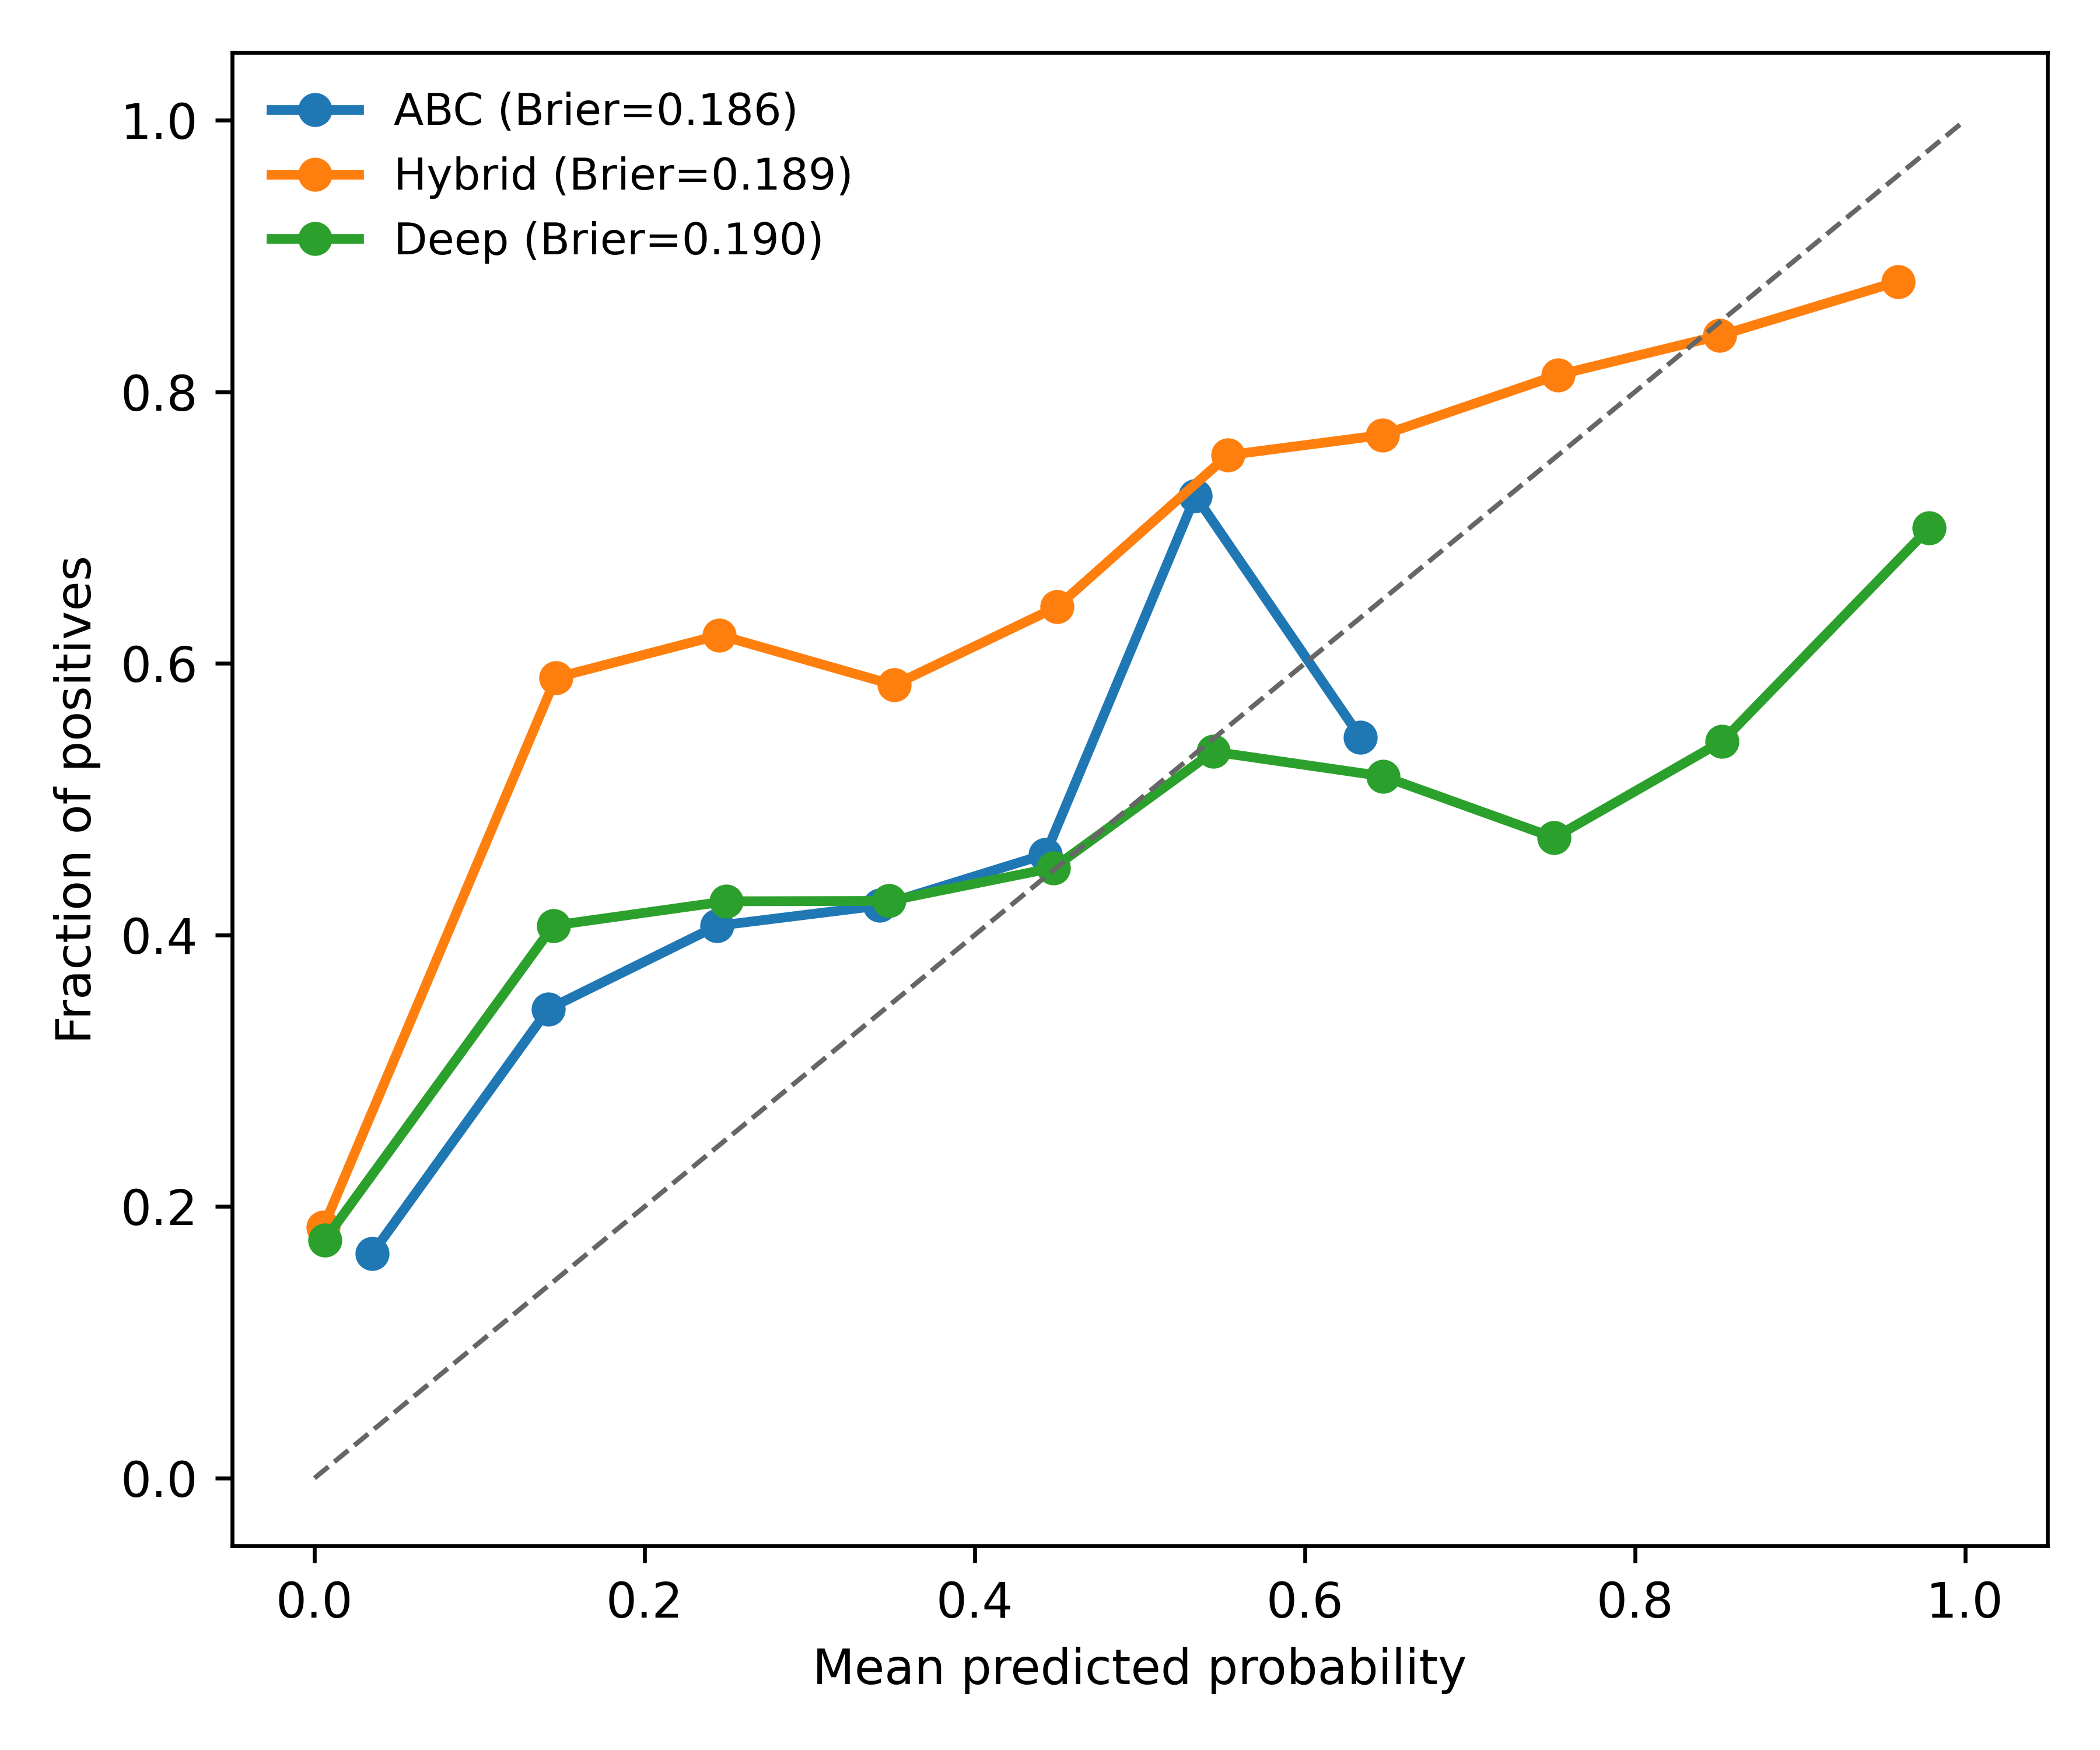
\includegraphics[width=\textwidth]{fig_curves_bcn_calibration.png}
\caption{Calibration.}
\end{subfigure}
\caption{Validation curves on the independent BCN20000 cohort. Model weights and decision thresholds were frozen from the HAM10000 training phase.}
\label{fig:curves_bcn}
\end{figure}

\begin{figure}[H]
\centering
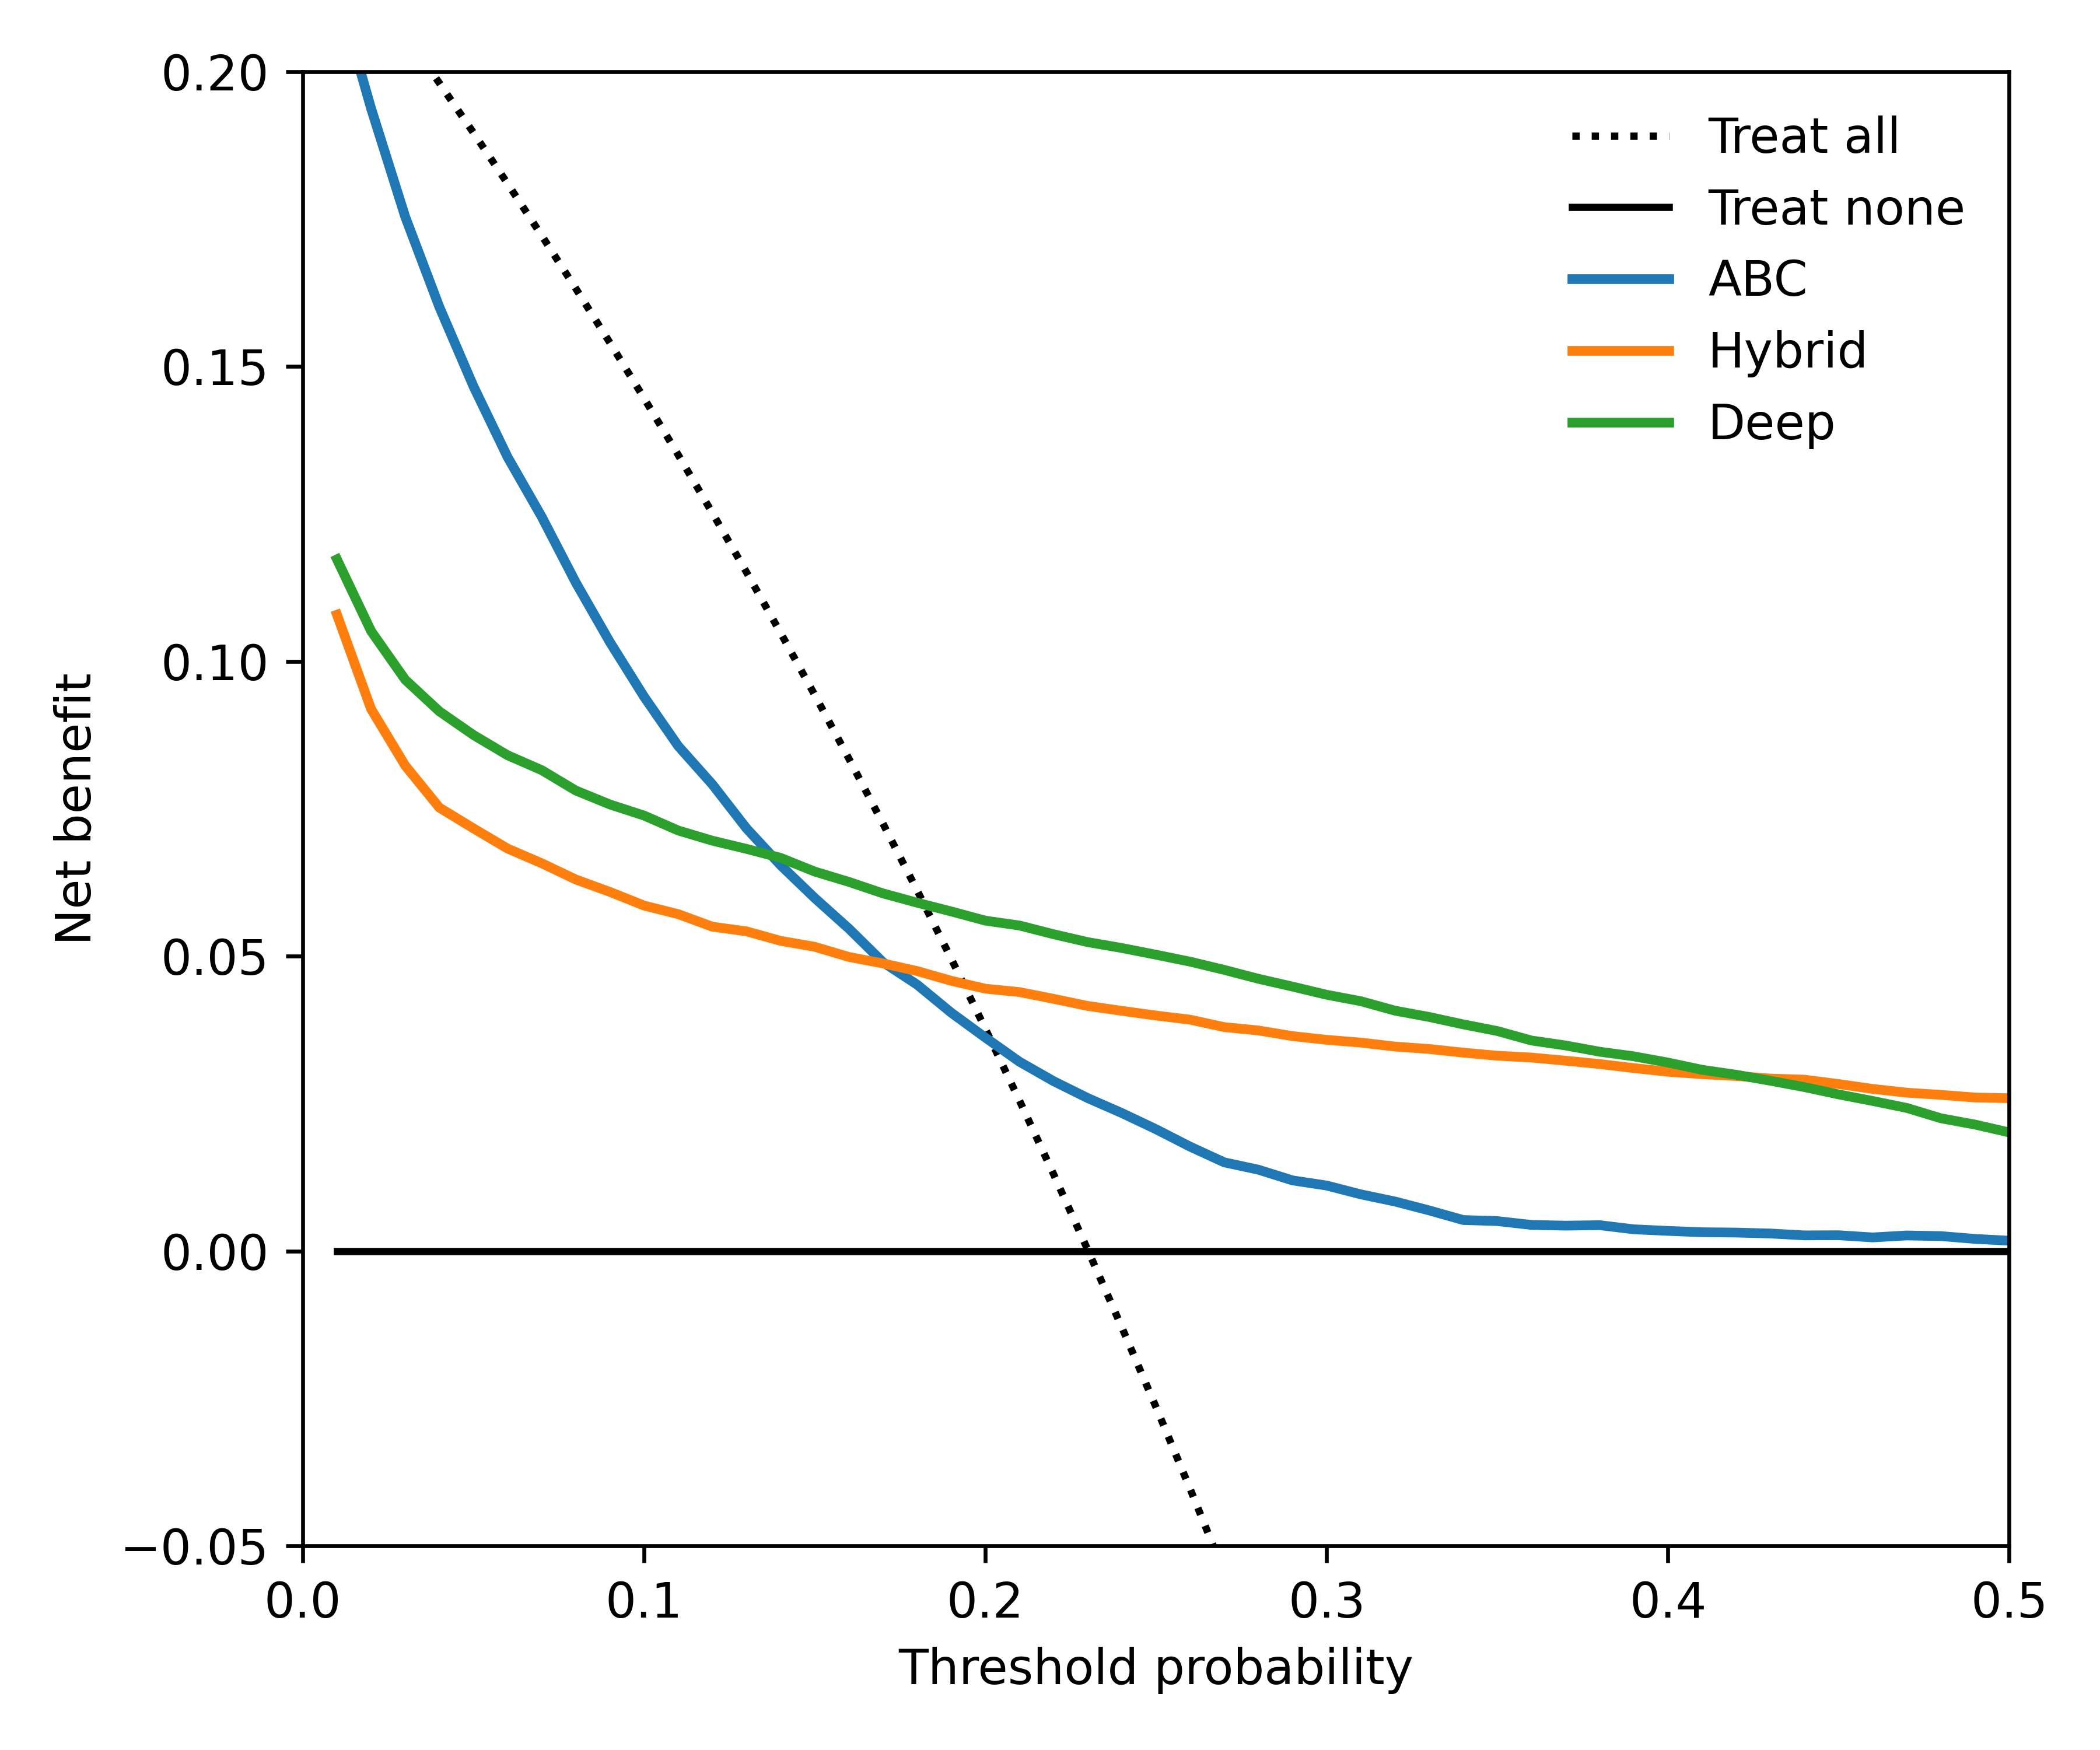
\includegraphics[width=0.95\textwidth]{fig_dca_bcn.png}
\caption{Decision-curve analysis on the independent BCN20000 cohort over threshold probabilities 0.02--0.50.}
\label{fig:dca_bcn}
\end{figure}

\subsection{Recalibration and decision-curve analysis}

Post-hoc recalibration was evaluated on both the HAM10000 test split and the external BCN20000 cohort. On the HAM10000 test split, Platt scaling and isotonic regression improved probability accuracy for both learned model families. Deep Brier score decreased from 0.097 to 0.074 with Platt scaling and 0.072 with isotonic regression. Hybrid Brier score decreased from 0.080 to 0.078 with Platt scaling and 0.073 with isotonic regression. AUC remained essentially unchanged, reinforcing that ranking performance and probability reliability are distinct model properties.

On HAM10000, ABC-conditioned calibration reduced Brier score relative to the raw deep score and reached the same Brier score as Platt scaling and isotonic regression. On BCN20000, ABC-conditioned correction improved over the raw deep score but did not outperform Platt scaling or isotonic regression in Brier score. However, because the transform depends on ABC descriptors, it can alter ranking; therefore, changes in ROC-AUC should be interpreted as post-hoc descriptor-conditioned score correction rather than conventional calibration.

\begin{table}[htbp]
\centering
\caption{HAM10000 recalibration summary.}
\label{tab:recalibration_ham}
\begin{tabular}{llrrrr}
\toprule
Model family & Probability scale & AUC & Brier & Slope & Intercept \\
\midrule
Deep & Raw & 0.887 & 0.097 & 0.261 & -1.047 \\
Deep & Platt & 0.887 & 0.074 & 0.896 & -0.197 \\
Deep & Isotonic & 0.886 & 0.072 & 0.742 & -0.344 \\
Hybrid & Raw & 0.885 & 0.080 & 0.439 & -0.151 \\
Hybrid & Platt & 0.885 & 0.078 & 0.884 & -0.199 \\
Hybrid & Isotonic & 0.880 & 0.073 & 0.575 & -0.538 \\
\bottomrule
\end{tabular}
\end{table}

Decision-curve analysis over threshold probabilities 0.02--0.50 showed threshold-dependent differences between the deep and hybrid models (Figure~\ref{fig:dca_ham}). The restricted threshold range and rescaled y-axis make model differences readable while retaining treat-all and treat-none reference strategies.

\begin{figure}[H]
\centering
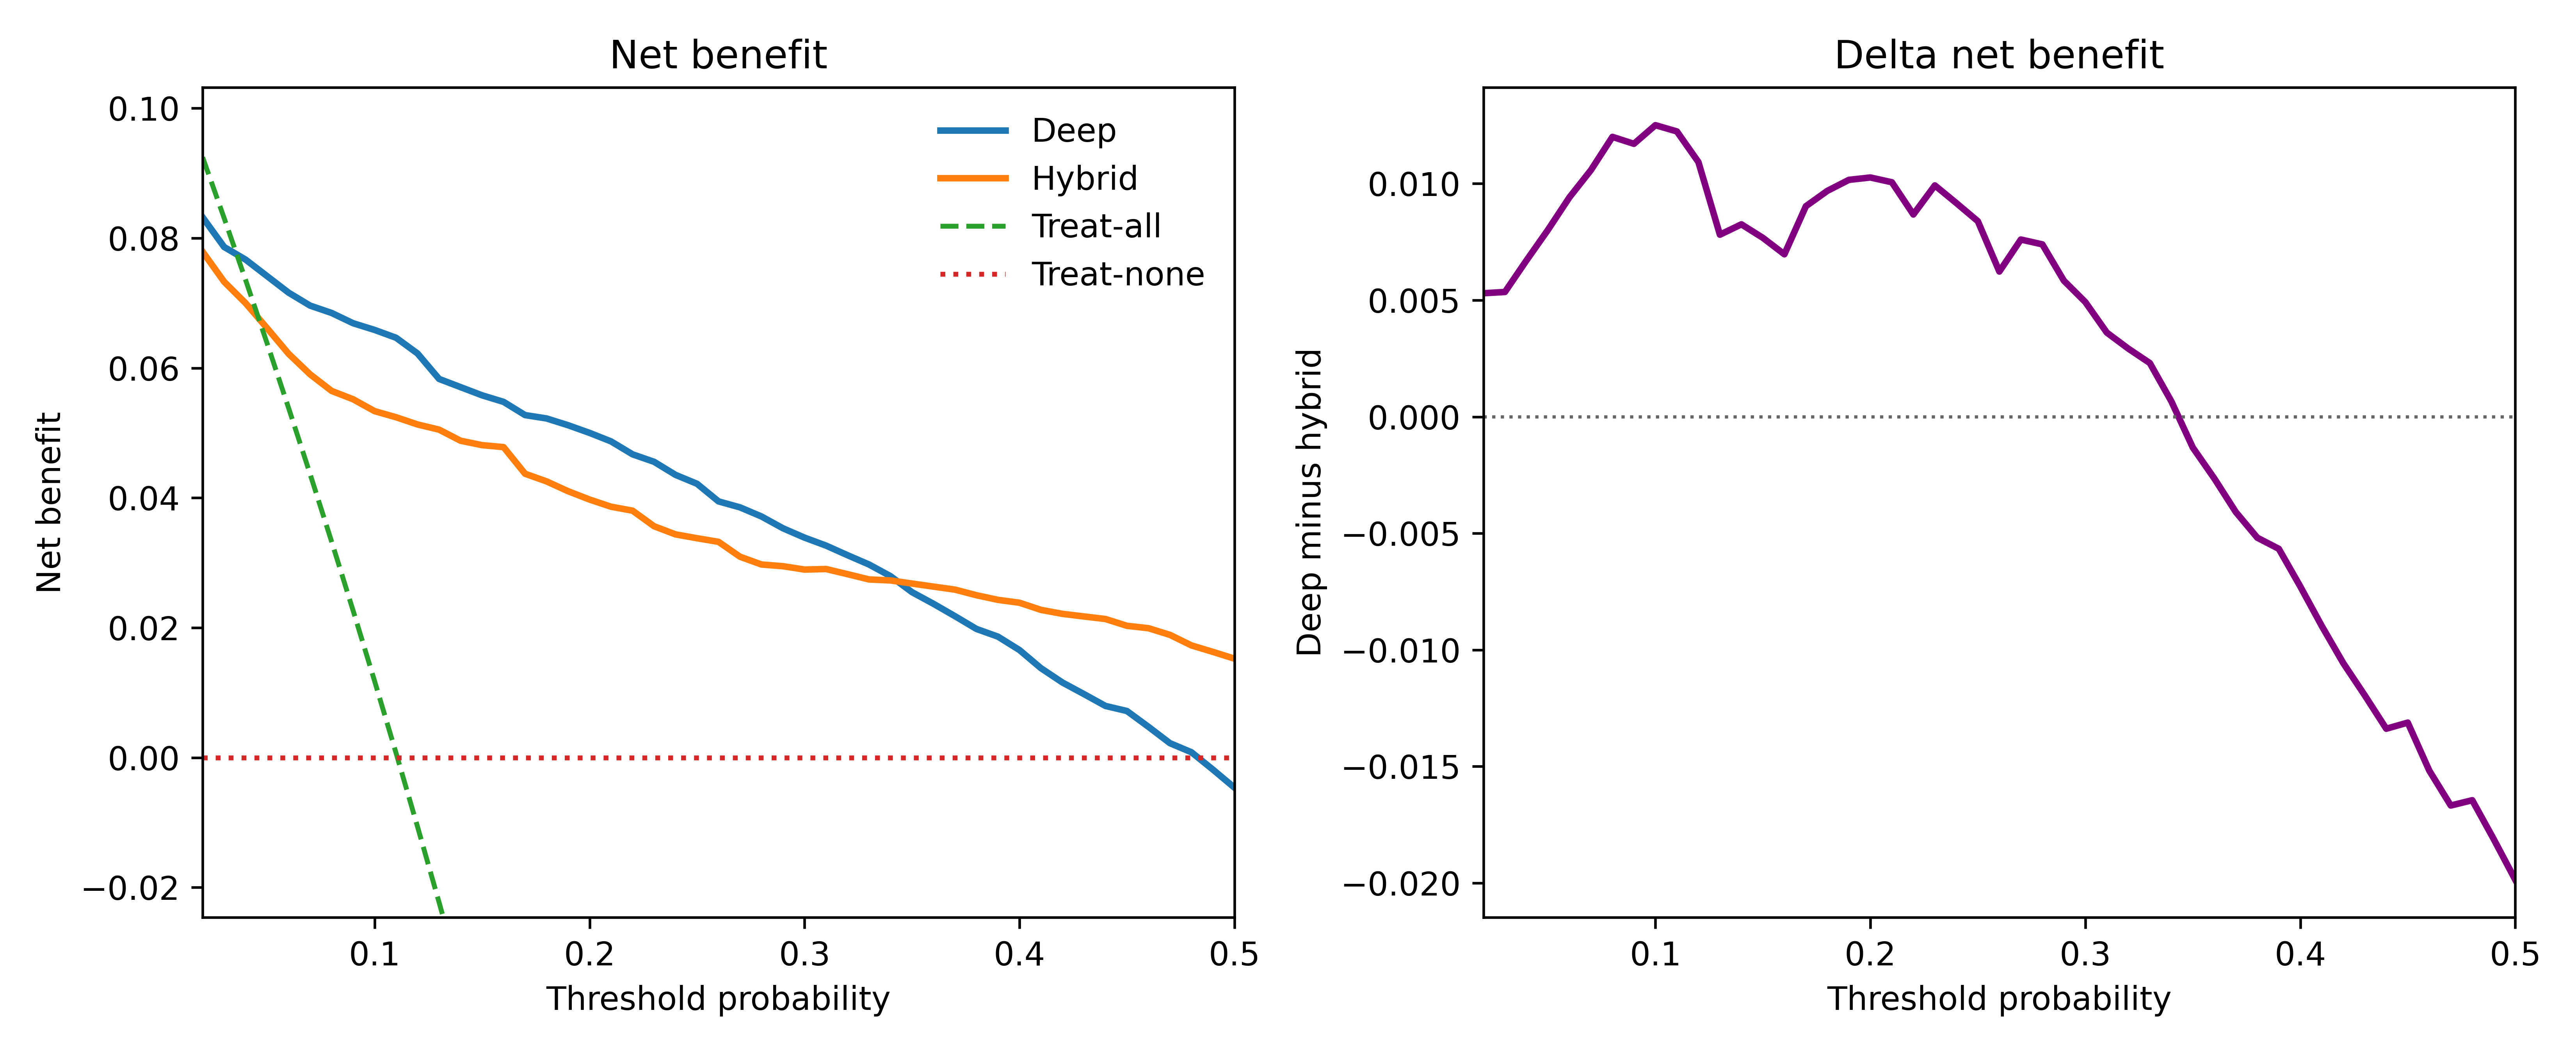
\includegraphics[width=0.95\textwidth]{fig_dca_ham.png}
\caption{Decision-curve analysis on HAM10000 test over threshold probabilities 0.02--0.50. The right panel shows net benefit difference (deep minus hybrid).}
\label{fig:dca_ham}
\end{figure}

\subsection{Implicit concept learning and subgroup calibration}

Linear probes trained on EfficientNet-B0 embeddings recovered several handcrafted descriptors, suggesting partial implicit encoding of classical concepts (Figure~\ref{fig:implicit}). Recoverability was strongest for HSV value statistics ($R^2 \approx 0.67$ for \texttt{C\_color\_mean\_v} and $R^2 \approx 0.60$ for \texttt{C\_color\_std\_v}), substantial for border irregularity and saturation mean, and poor for asymmetry. These results help explain why explicit descriptor fusion did not materially improve discrimination over embeddings-only XGBoost.

\begin{figure}[H]
\centering
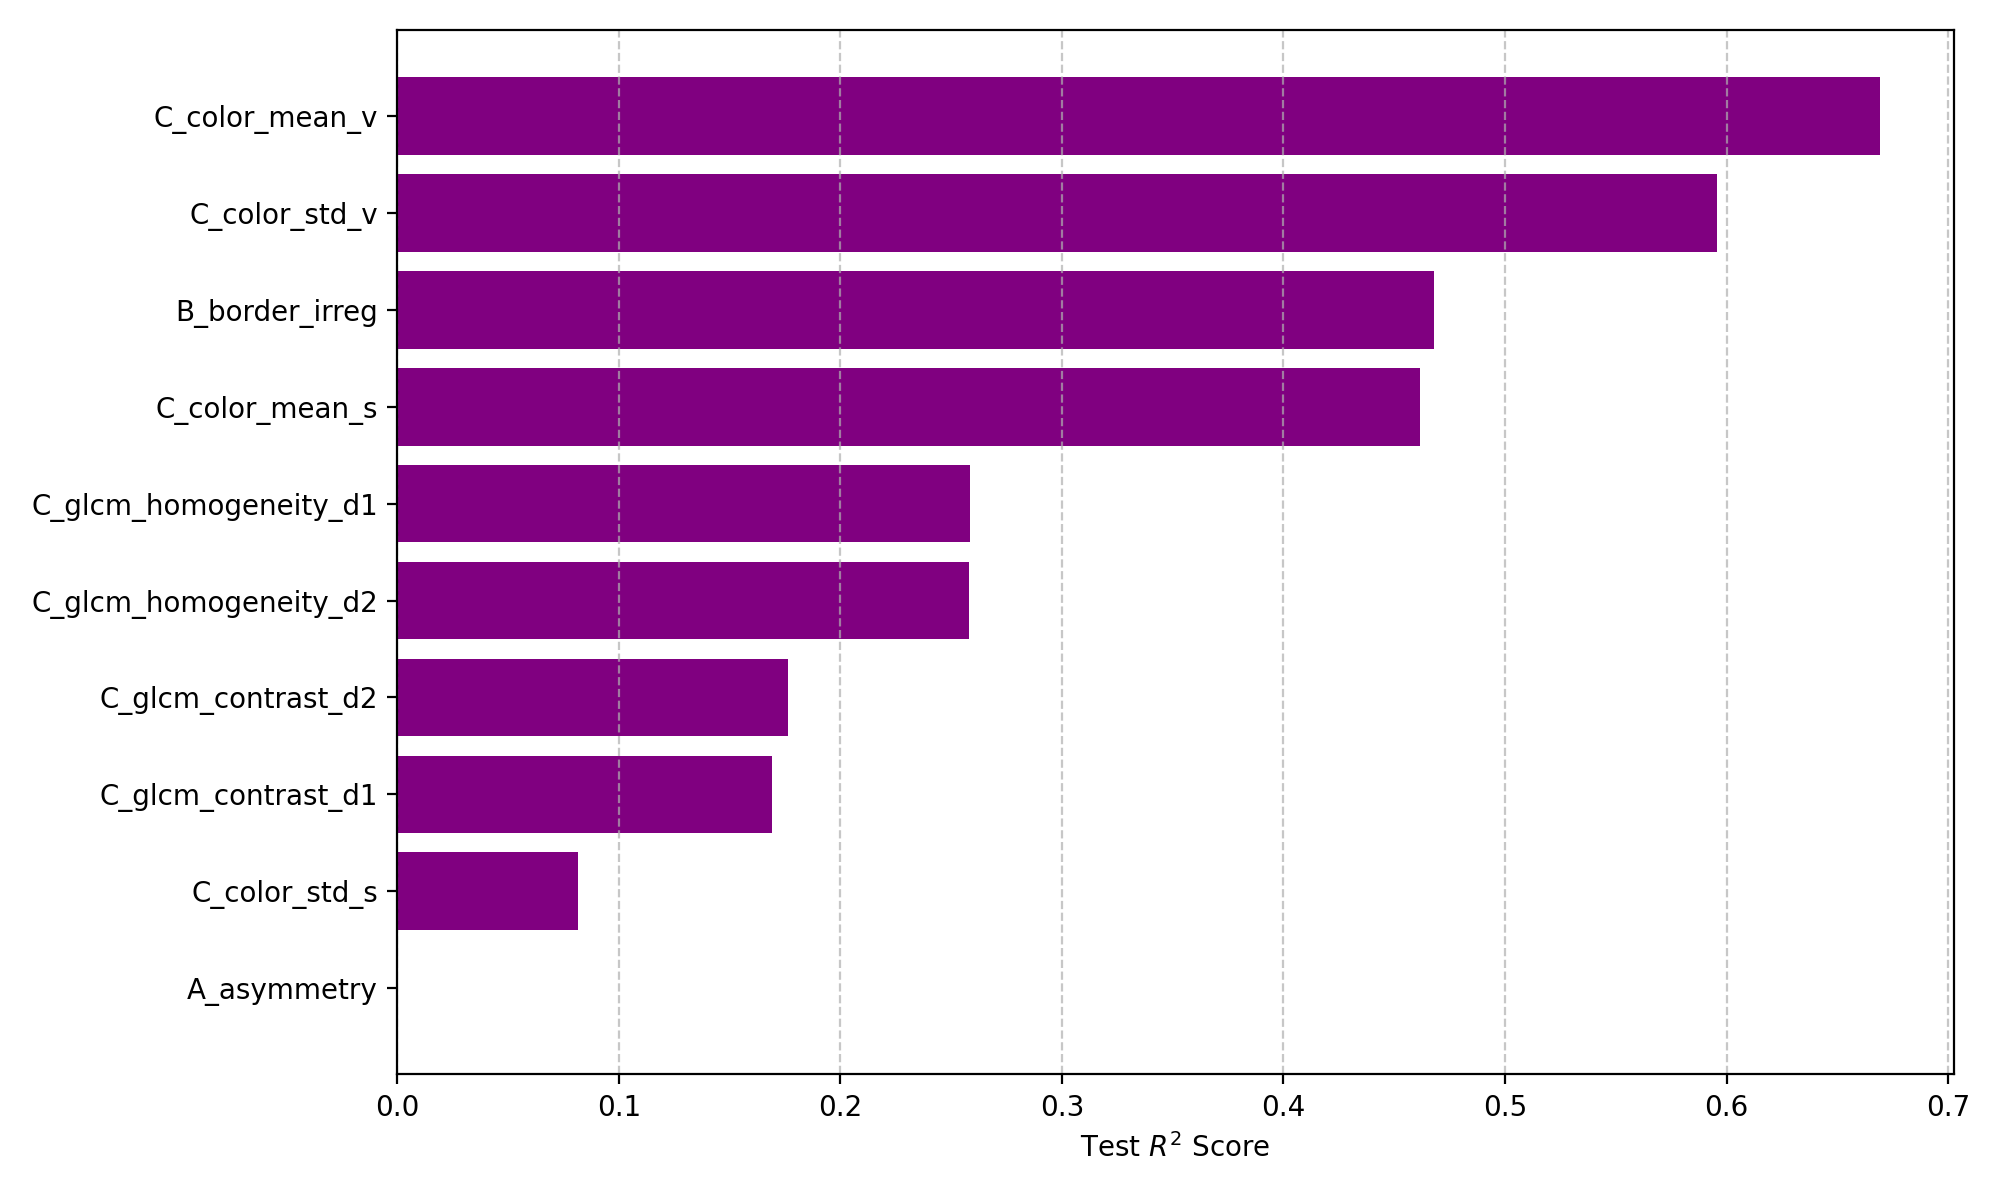
\includegraphics[width=0.85\textwidth]{fig_implicit_concept_learning.png}
\caption{Implicit concept learning. Linear Ridge probes reconstruct handcrafted descriptors from EfficientNet-B0 embeddings; bars show test-set $R^2$.}
\label{fig:implicit}
\end{figure}

Calibration quality varied across demographic strata in descriptive subgroup analysis (Figure~\ref{fig:subgroup}). These analyses were not designed as formal fairness tests but identify subgroup-level calibration checks as a useful component of model auditing.

\begin{figure}[H]
\centering
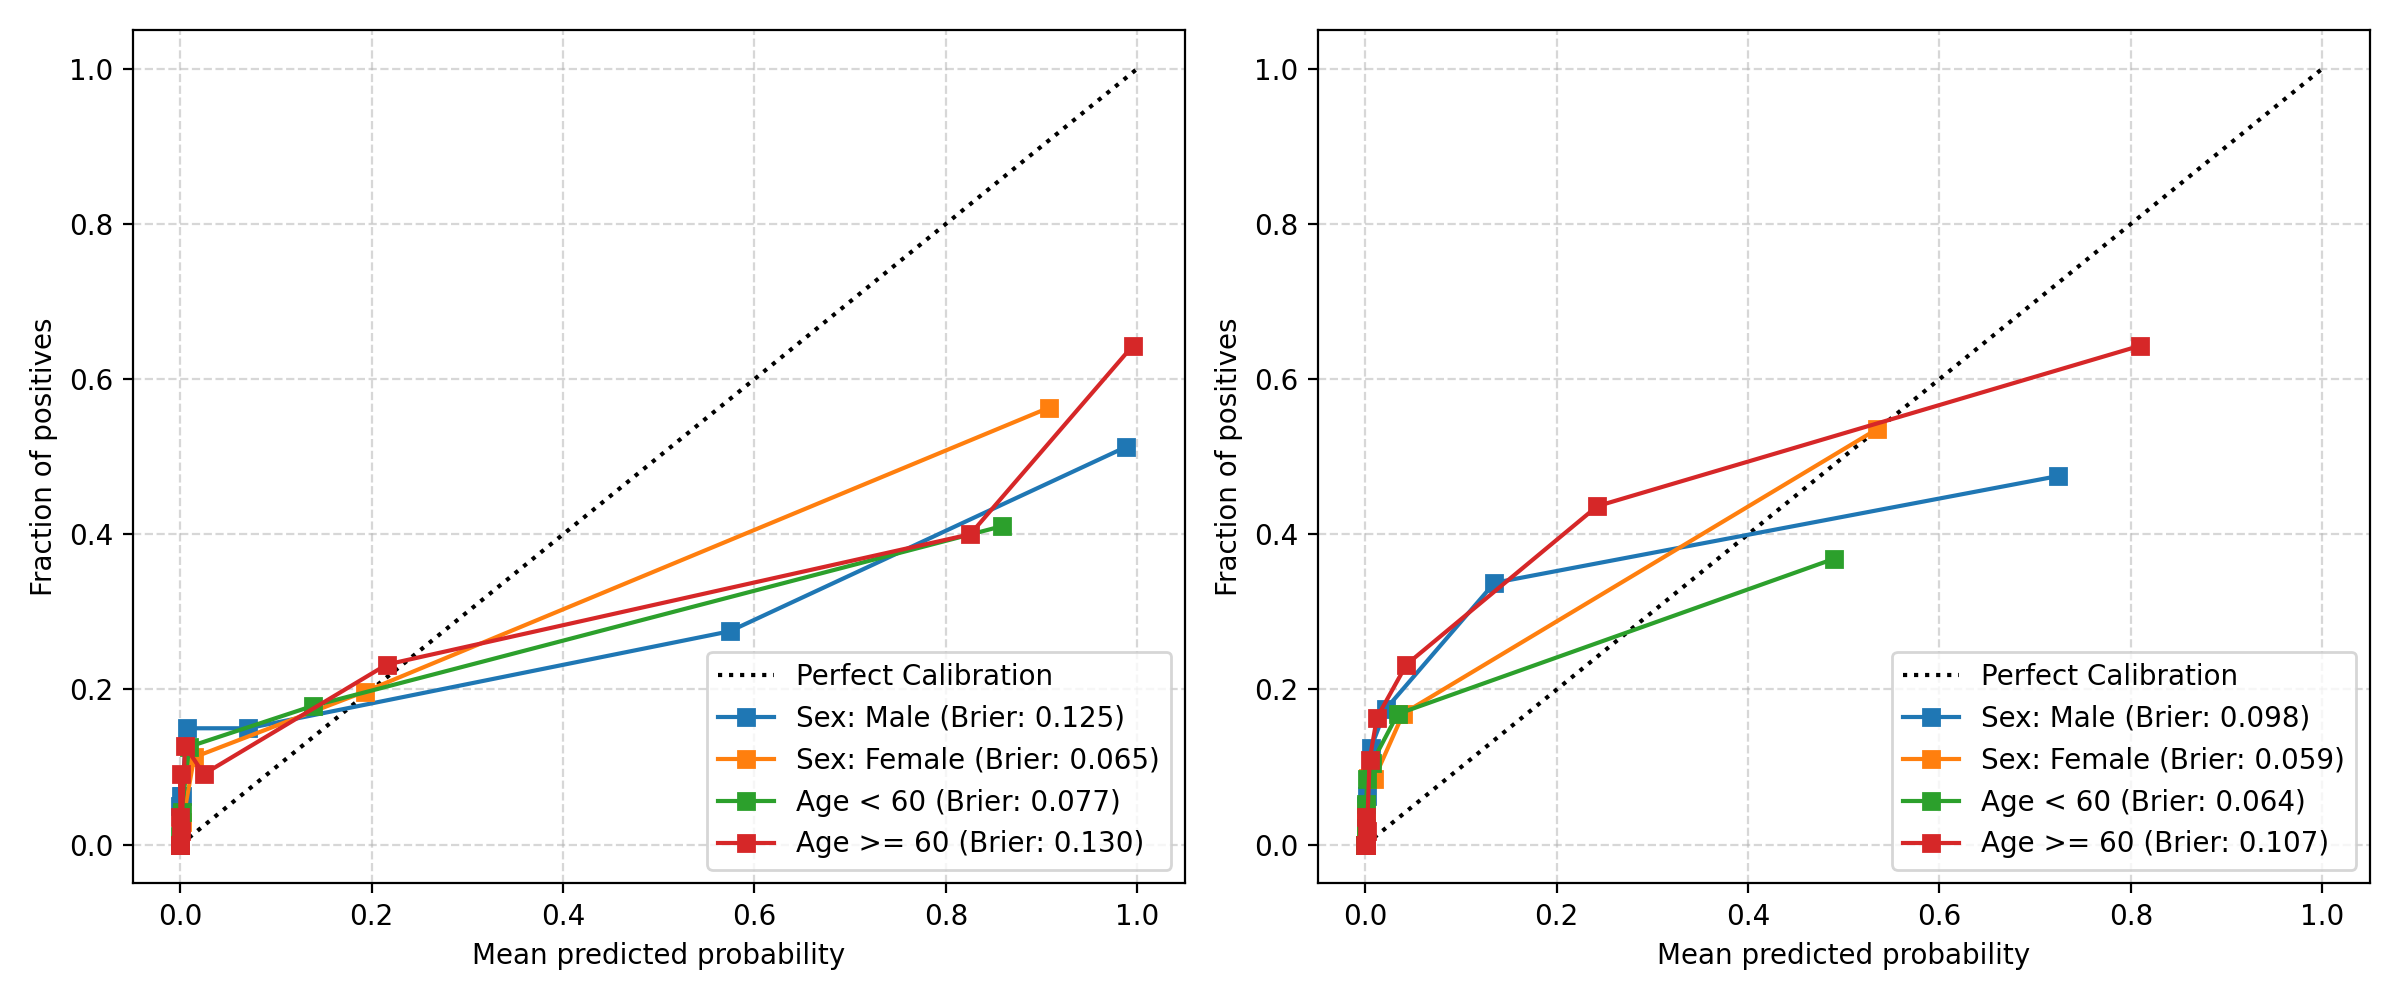
\includegraphics[width=0.95\textwidth]{fig_subgroup_fairness.png}
\caption{Subgroup calibration heterogeneity on HAM10000 by sex and age strata.}
\label{fig:subgroup}
\end{figure}

\subsection{Feature and image-level explainability}

SHAP-style contributions for tree-based models identified asymmetry, border irregularity, and HSV intensity descriptors as clinically interpretable drivers in descriptor-level analyses (Figure~\ref{fig:shap}). In the hybrid model, block-wise aggregation showed that EfficientNet embeddings dominated total contribution magnitude, while ABC descriptors contributed a small but auditable component. Feature-ranking stability between HAM test and the secondary Task 3-label set was high, but this should be interpreted within the shared-image-corpus limitation.

\begin{figure}[H]
\centering
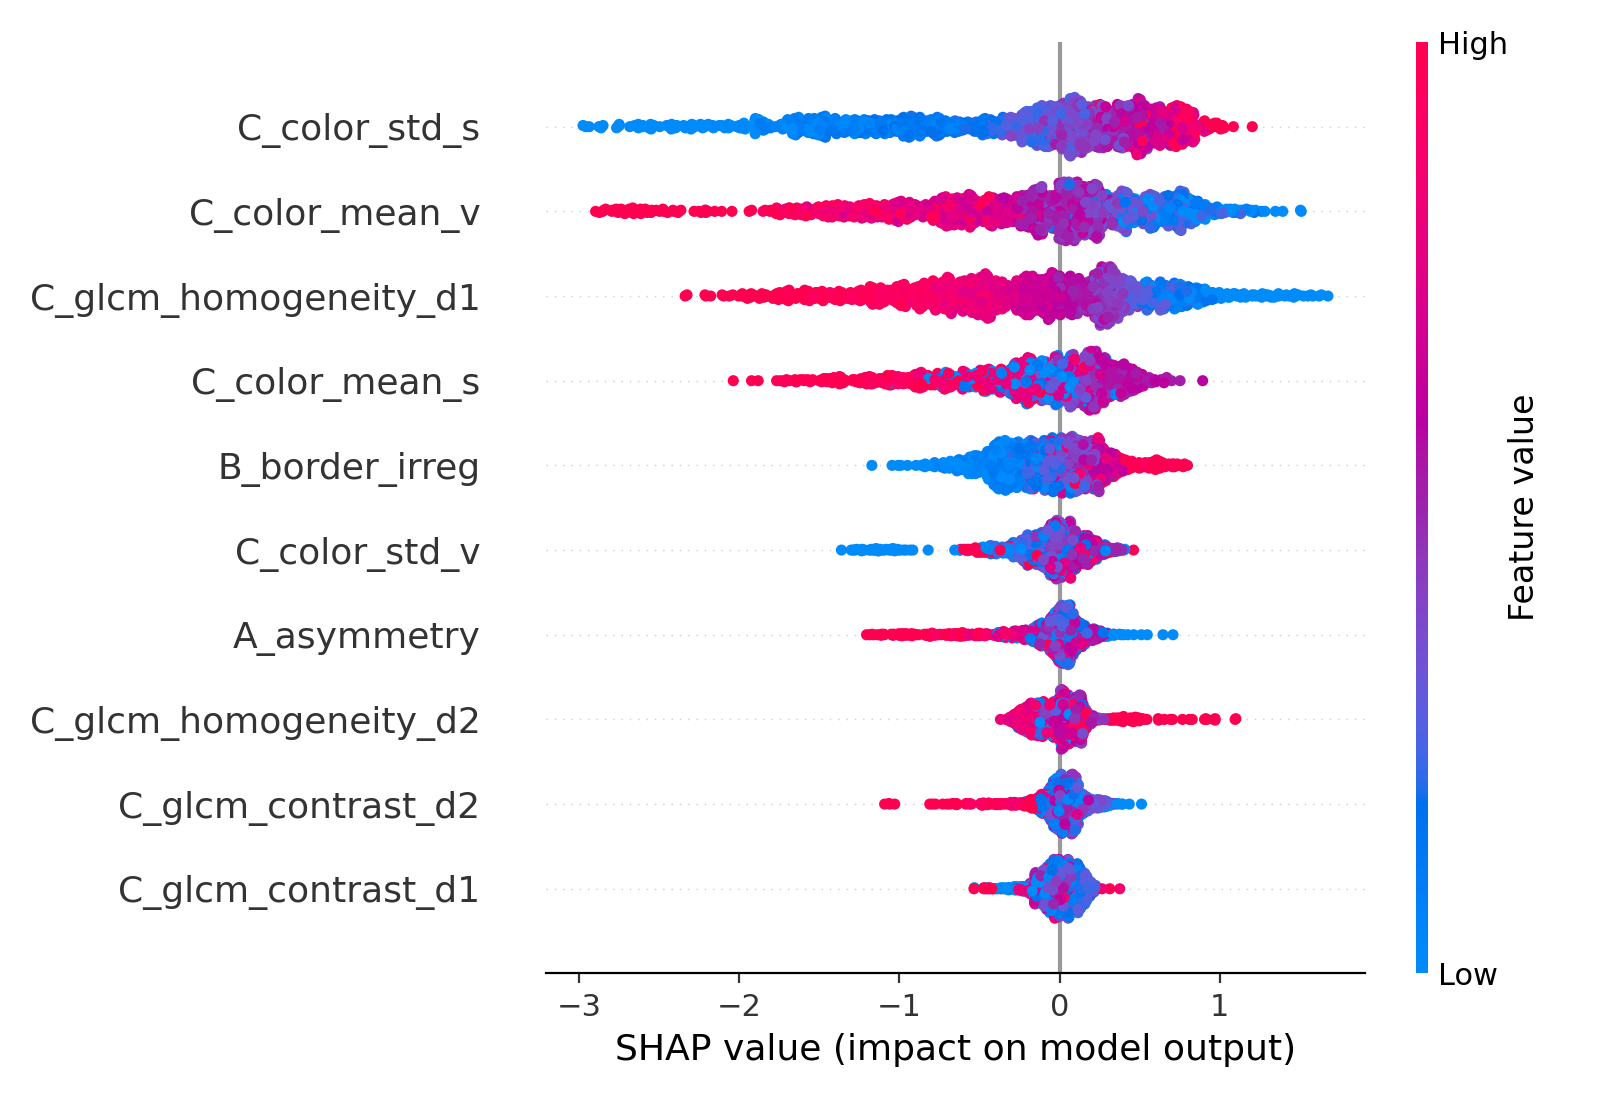
\includegraphics[width=0.90\textwidth]{fig_shap_summary.png}
\caption{SHAP-style summary plot for the handcrafted ABC model.}
\label{fig:shap}
\end{figure}

Grad-CAM overlays for non-degenerate examples showed attention concentrated on lesion regions in selected high-confidence melanoma cases (Figure~\ref{fig:gradcam}). These examples support qualitative error auditing but should not be interpreted as a quantitative localization validation.

\begin{figure}[H]
\centering
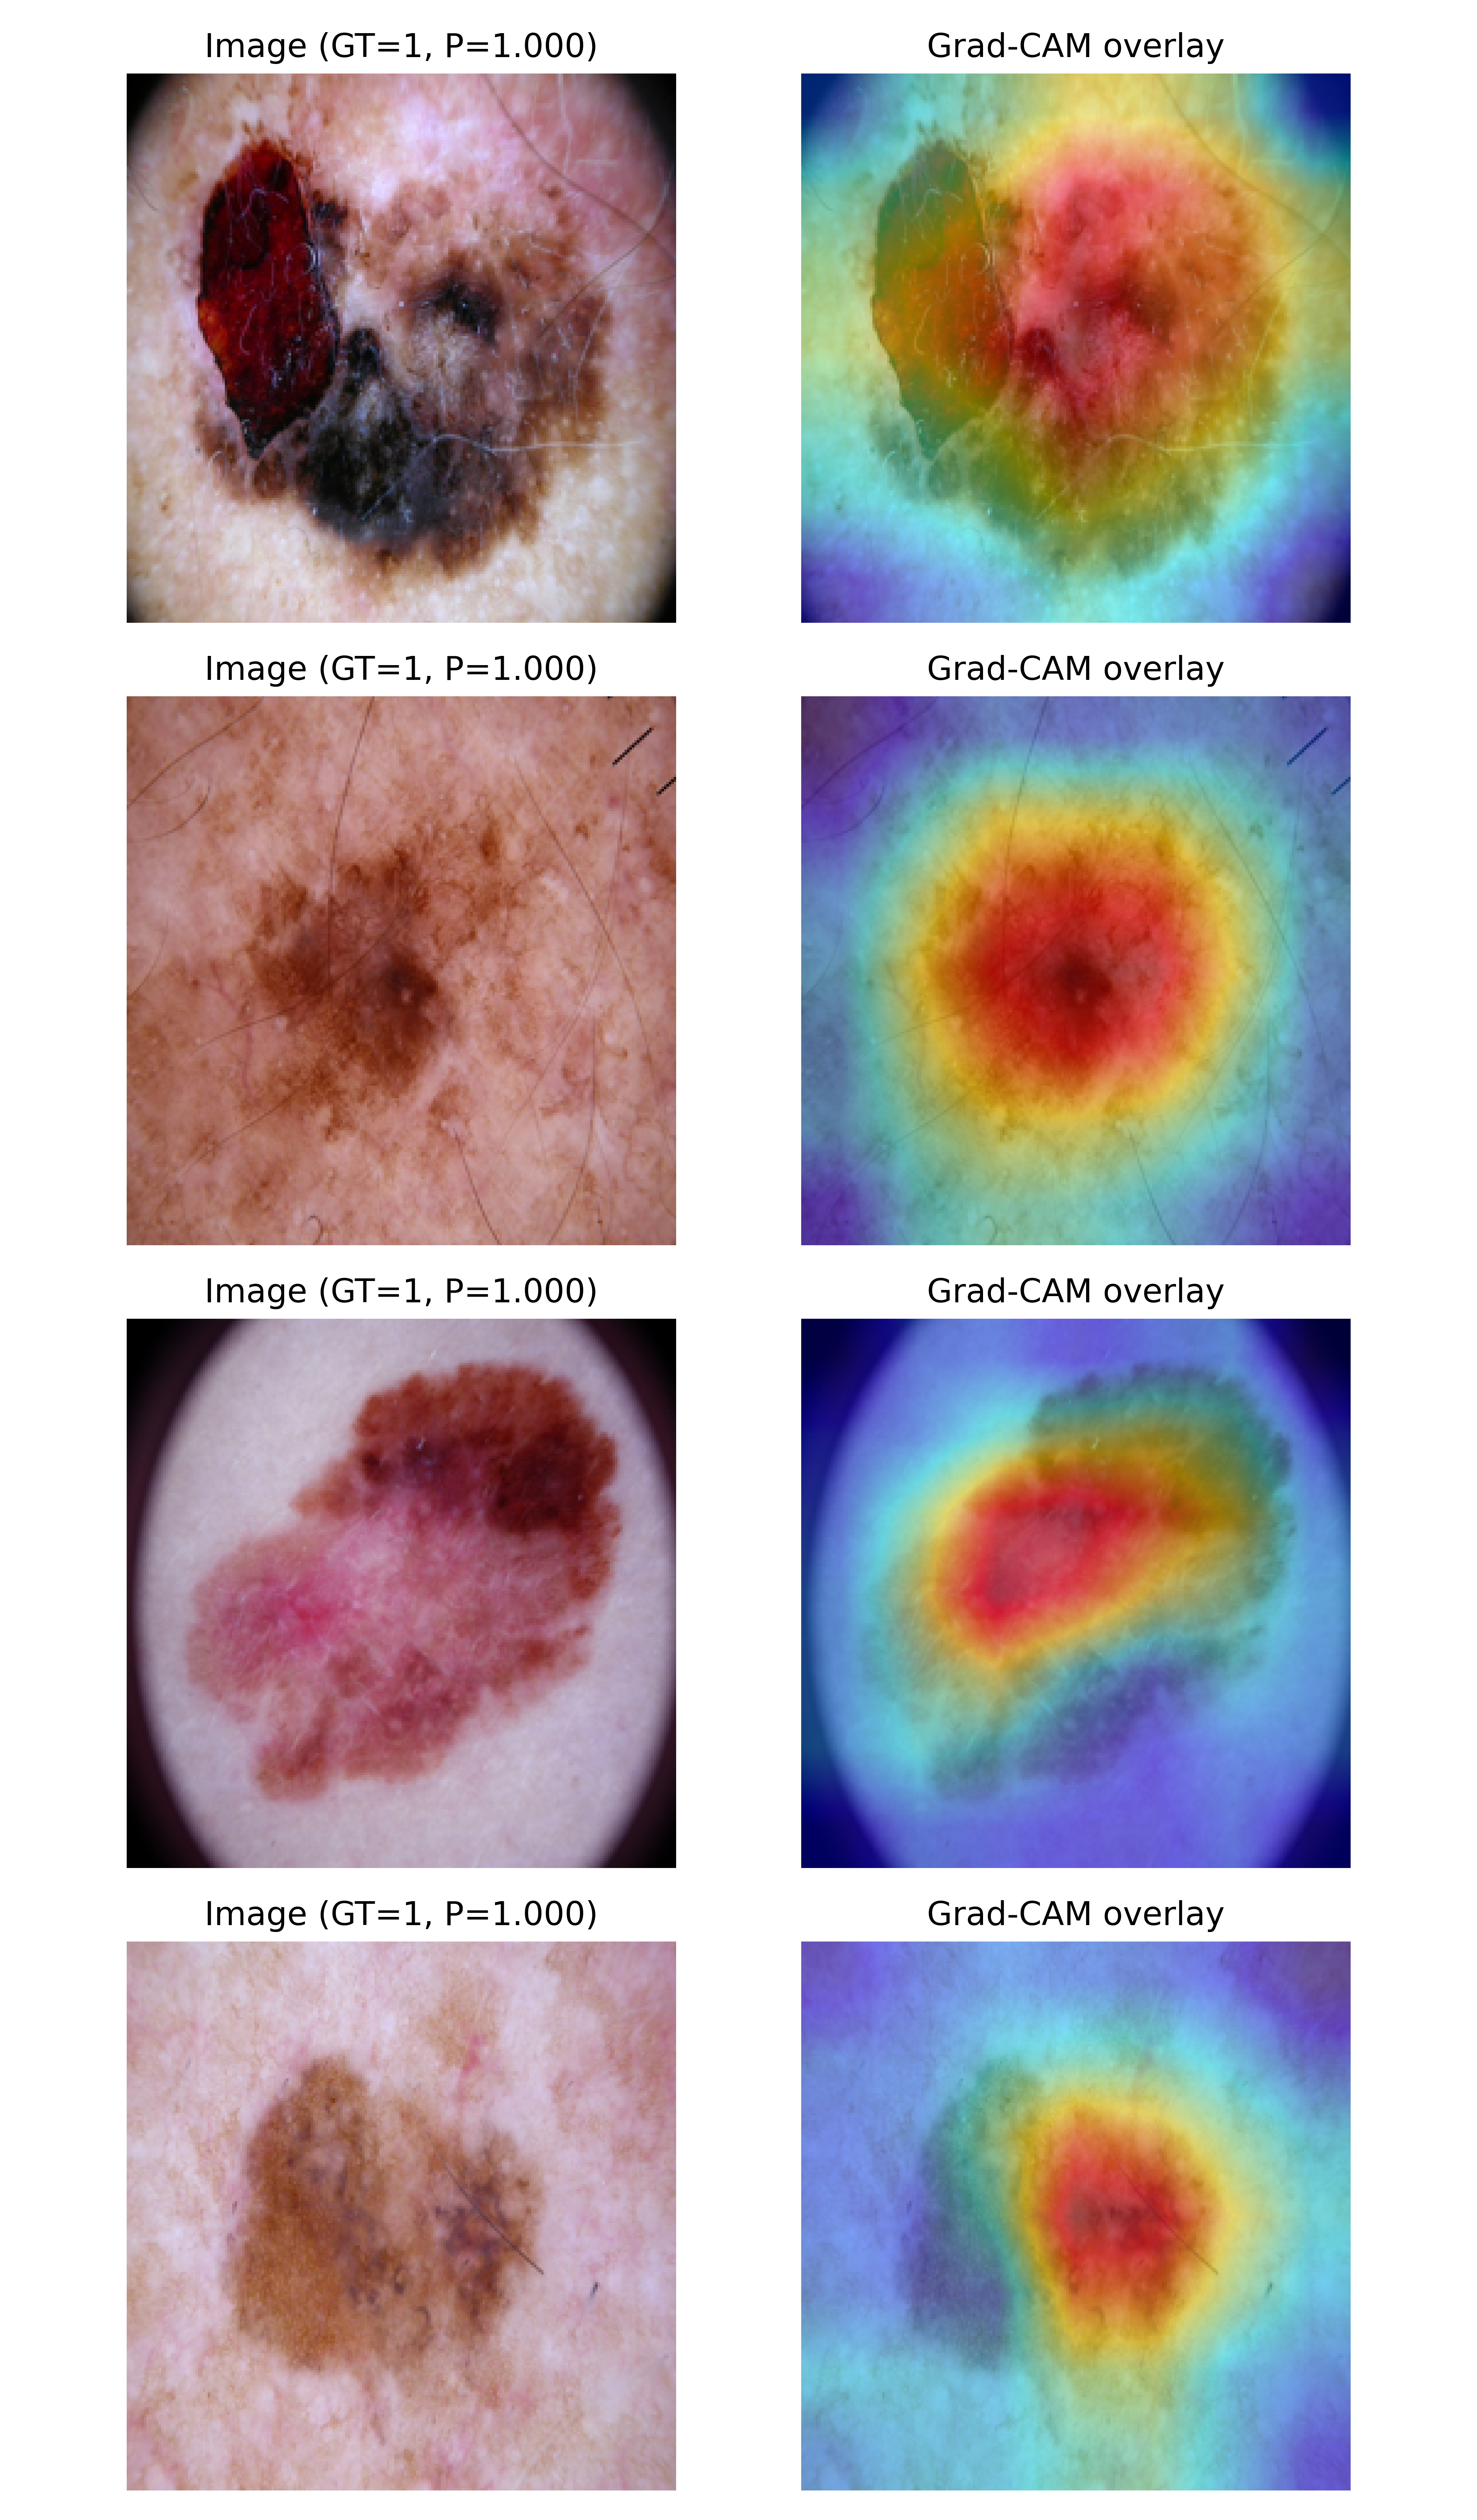
\includegraphics[width=0.82\textwidth]{fig_gradcam_cases.png}
\caption{Grad-CAM overlays for selected non-degenerate deep-baseline examples.}
\label{fig:gradcam}
\end{figure}

\section{Discussion}

The revised analysis resolves two central methodological risks: endpoint inconsistency and unsupported claims about independent validation. The melanoma-only endpoint aligns the HAM10000 labels with the stated clinical task and with the official Task 3 melanoma label. The provenance audit shows that the available Task 3 files are not a separate cohort in this workspace, so conclusions from Task 3 are restricted to within-corpus behavior. Crucially, the addition of the BCN20000 cohort, enforced via strict perceptual hash auditing, supplies the missing independent external validation and proves that the hybrid and deep representations are transportable across dermoscopic image distributions without retraining.

Under lesion-level separation, the deep and hybrid models had similar ROC discrimination, but calibration favored the hybrid model under raw probabilities. Recalibration improved Brier score for both learned model families without materially changing AUC, consistent with the view that discrimination and probability accuracy should be assessed separately \citep{vancalster2025performance}. Decision-curve analysis further demonstrated that threshold-specific utility can differ even when discrimination is similar. 

The ABC-conditioned model provides algorithmic novelty by allowing segmentation-derived descriptors to modulate the post-hoc transformation of deep logits. The external BCN20000 results suggest that this descriptor-conditioned correction can partially recover ranking performance under domain shift, but its calibration performance did not exceed global Platt or isotonic recalibration. Thus, the method is promising as a lightweight interpretable score-correction layer, but further regularization and validation are needed before claiming superior calibration.

The ablation analysis indicates that embeddings account for most predictive signal. Handcrafted ABC descriptors did not improve discrimination when concatenated to embeddings, but they provide an explicit concept channel for audit and interpretation. The implicit-concept probes clarify this behavior: several color and border descriptors are already linearly recoverable from the EfficientNet embedding space, whereas asymmetry is not.

The secondary Task 3-label analysis is useful for label-harmonization and full-corpus reporting, but it does not answer whether the models generalize to non-overlapping data. A future cohort could support that claim only after a documented zero-overlap audit by image identifier and lesion identifier where available.

\section{Limitations}

The study uses retrospective public data and a within-corpus evaluation design. Patient-level identifiers are not consistently available in HAM10000, so splitting was enforced at the lesion level. Although this prevents images from the same lesion crossing splits, residual patient-level dependence cannot be fully excluded.

The segmentation pipeline uses classical methods and handcrafted descriptors whose quality depends on mask quality. Grad-CAM is reported qualitatively and does not establish quantitative localization accuracy. Subgroup calibration analyses are descriptive and may be influenced by subgroup sample-size imbalance.

Most importantly, while the local ISIC 2018 Task 3 files overlap completely with HAM10000, our inclusion of the BCN20000 external validation cohort circumvents this limitation. However, differences in underlying demographic sampling between HAM10000 and BCN20000 could still introduce unmeasured transportability variance.

\section{Conclusion}

We present a reproducible audit framework for melanoma-only dermoscopic classification. The framework harmonizes endpoint definition, documents dataset provenance, enforces lesion-level separation, and evaluates discrimination, calibration, recalibration, decision utility, and interpretability as distinct model properties. The revised results show similar internal discrimination between deep and hybrid models, better raw Brier score for the hybrid model, and meaningful probability improvements after recalibration. Furthermore, independent validation on the zero-overlap audited BCN20000 cohort confirmed the external transportability of the models. The framework is intended to support transparent model auditing while clearly establishing evidence of true external generalization.

\section*{Code and Data Availability}

Submission is blocked until the forthcoming Zenodo DOI is inserted here. The archived release is expected to contain the full experimental pipeline for segmentation benchmarking, handcrafted feature extraction, deep model training, embedding extraction, hybrid model training, lesion-level testing, secondary Task 3-label evaluation, bootstrap analyses, calibration estimation, and decision-curve analysis.

All experiments are reproducible using the fixed random seeds and configuration files included in the repository. The release also includes the seeded ISIC 2018 Task 1 subset identifiers used in the segmentation benchmark and the derived result files produced by the pipeline.

HAM10000 and ISIC 2018 datasets are publicly available from the International Skin Imaging Collaboration and must be obtained directly from their official repositories in accordance with their respective data use agreements.

\section*{Reproducibility}

All experiments used fixed configuration files and random seed 42. Model architectures, hyperparameters, preprocessing settings, and split definitions are specified in the repository.

\section*{Declaration of Competing Interest}
The authors declare no competing interests.

\section*{Funding}
This work was supported by the Conselho Nacional de Desenvolvimento Científico e Tecnológico (CNPq) under Grant No.~309589/2023-1 and by the Coordenação de Aperfeiçoamento de Pessoal de Nível Superior (CAPES).

\section*{Ethics Approval}
This study used publicly available, de-identified datasets (HAM10000 and ISIC 2018); ethical approval and informed consent were not required.

\section*{Data Availability}
HAM10000 and ISIC 2018 Task 3 datasets are publicly available from the International Skin Imaging Collaboration.

\section*{CRediT Authorship Contribution Statement}
Rafael Oliveira Chaves: Conceptualization, Methodology, Software, Formal analysis, Writing -- Original Draft.
Antonio Pereira Junior: Supervision, Validation, Writing -- Review \& Editing.

\bibliographystyle{elsarticle-num}
\bibliography{references}

\end{document}
